\documentclass[a4paper,12pt]{article}

\usepackage[unicode]{hyperref}
\usepackage{cmap}
\usepackage[T2A]{fontenc}
\usepackage[utf8]{inputenc}


\usepackage[verbose,dvips,a4paper,tmargin=20mm,bmargin=20mm,lmargin=20mm,rmargin=20mm,headsep=4pt,includeheadfoot]{geometry}

\usepackage[nodisplayskipstretch]{setspace}
\usepackage{amsmath}
%\usepackage{mathenv}
\usepackage{mathtools}
\usepackage{indentfirst}
\usepackage{titling}

\usepackage{txfonts} % use before local fonts - only for math
%\usepackage{dejavu}
\usepackage{atu_csb}
\usepackage{atu_ofs}
\usepackage{atu_nim}

\usepackage{graphicx}
\usepackage{placeins} % FloatBarrier
\usepackage{siunitx}

\usepackage[backend=biber,sorting=none,maxnames=100,bibstyle=gost-numeric,babel=other]{biblatex}
%\usepackage[backend=biber,sorting=none,maxnames=100]{biblatex}

\usepackage{tikz}
\usetikzlibrary{arrows}
\usetikzlibrary{patterns}

\usepackage{blox}
\usepackage[europeanresistors,americaninductors,siunitx,fulldiodes]{circuitikz}

\usetikzlibrary{calc}
\usetikzlibrary{arrows}
\usetikzlibrary{patterns}
%\usepgflibrary{shapes.geometric}
\usetikzlibrary{external}


\definecolor{haircolor}{rgb}{0.7,0.7,1.0}
\newcommand{\TikzAddPadding}{\path (current bounding box.north east) ++(+0.1,+0.1); \path (current bounding box.south west) ++(-0.1,-0.1);}

\tikzset{
  >=stealth,
  %semiRed/.style={fill=red,opacity=0.3,draw=black,thin},
  hair/.style={draw,color=haircolor,line width=0.1pt},
  medline/.style={draw=black,line width=0.6pt},
  medlinep/.style={draw=black,line width=0.6pt,->},
  semiboldline/.style={draw=black,line width=1.2pt},
  semiboldlinep/.style={draw=black,line width=1.2pt,->},
  infoline/.style={draw=gray,line width=1.4pt},
  boldline/.style={draw=black,line width=2.0pt},
  boldlinep/.style={draw=black,line width=2.0pt,->},
  wire/.style={draw=black,line width=1.0pt},
  elelem/.style={draw=black,line width=1.5pt},
  subelem/.style={draw=black,dashed,line width=0.6pt}
}


\usepackage[europeanresistors,americaninductors,siunitx,fulldiodes]{circuitikz}

\usepackage[english,ukraineb,russian]{babel}
%\usepackage[margin=10pt,font=small,labelfont=bf,labelsep=endash]{caption} % format=hang|plain...

\usepackage{currfile}

\setcounter{topnumber}{3}
\renewcommand\topfraction{.7}
\setcounter{bottomnumber}{2}
\renewcommand\bottomfraction{.6}
\setcounter{totalnumber}{7}
\renewcommand\textfraction{.1}
\renewcommand\floatpagefraction{.5}
\setcounter{dbltopnumber}{2}
\renewcommand\dbltopfraction{.7}
\renewcommand\dblfloatpagefraction{.6}

\clubpenalty9500
\widowpenalty9500%


\newlength{\TW}
\setlength{\TW}{0.01\textwidth}

\DeclareMathOperator*{\sign}{sign}

\title{Идентификация хаотических систем}
\author{А.И.~Гуда}

%\DeclareFieldFormat{titlecase}{xxx #1 xxx}
\addbibresource{atuworks.bib}
\addbibresource{artrefs.bib}

\hypersetup{
  pdftitle={\thetitle},
  pdfauthor={\theauthor},
  colorlinks=true,
  linkcolor=blue,
  citecolor=brown
}

% \linespread{1.3} setspace must be better
% \onehalfspacing
\setstretch{1.2}

\newcommand{\LinkRef}[1]{ \textit{\color{red}#1} }
\newcommand{\Cmt}[1]{ {\small\color{red}#1} }


\begin{document}

% \maketitle
%{ \tiny \verb! ~/proj/id_data/text/tasks.tex! }
{ \tiny \currfilepath }

\sloppy

\tableofcontents

\nocite{*} % debug literature

\section{Определение идентификации}

\subsection{История}

\Cmt{Предельные случаи: Заде, Райбман.}

L.A.~Zadeh (1956), ``On the Identification Problem,''
IRE Transactions on Circuit Theory, 3, pp.  277--281.

More: Eykhoff, Rastrigin.

\subsection{Новые определения}

\Cmt{Привязка к текущей задаче, физика.}

\Cmt{Разные определения для разных задач или свести к одному определению?}

\subsection{Критерии идентификации}

\subsubsection{Отличие задачи идентификации от поиска экстремума}

На первый взгляд, при заданном критерии идентификации, задача идентификации
сводится к классической задаче описка экстремума: надо найти такие значения
параметров, при которых критерий принимает максимальное значение.
На самом деле, существуют определённые аспекты, которые делают такое
сведение практически невозможным.

Прежде всего, в задаче поиска
экстремума предполагается, что наблюдаемая система статична:
значение критерия не зависит от времени, и проведя измерение
в точке один раз, можно к нему не возвращаться.
Напротив, идентификация динамической системы предполагает,
что значение критерия, даже после какого-либо усреднения на конечном
интервале времени, есть величина динамическая, причём динамика определяется
не только параметрами системы, но и свойствами самой системы измерения,
а также процессом взаимодействия системы измерения с моделями. При этом
возможны весьма нетривиальные результаты, такие как параметрический
резонанс, распространение параметрических волн на множестве моделей и т.д.

Также существенную роль могут играть как шумы измерения, так и побочные
эффекты от процесса фильтрации шумов. Большая часть фильтров приводит к запаздыванию
в процессе измерения, и игнорирование этих явлений может привести
к нарушению устойчивости поиска.

В задаче поиска экстремума предполагается, что не только
значение функции известно точно в каждой точке, но также известны все производные.
В реальные задачах идентификации производные непосредственно
не доступны для измерения, а их оценка требует применения специальных
методов. При этом процесс оценивания производных, как правило,
более чувствителен к шумам измерения, чес собственно измерение.

Далее, в в задачах поиска экстремума не учитывается возможность
смещения экстремума со временем. Напротив, в задачах идентификации
или же изначально предполагается вариабельность параметров, или же
имеются ограничение на время измерения.


Все эти явления делают задачу идентификации более сложной, чем
классическая задача поиска экстремума, чем и обусловлено
существование широкого спектра методов идентификации. Тем не менее,
некоторые алгоритмы, применимые при поиска экстремума, могут быть
полезны при синтезе системы идентификации.






\subsubsection{Измеримые интегральные характеристики сигнала}

\Cmt{Откуда брать.}


\subsection{Тестовые системы (хаотические)}


\FloatBarrier
\subsection{Система Лоренца} % _LOR_

\LinkRef{
  lor: ASAU-22, 23, 24, 25, 26. APIR-2012. CSIT-2015. ISDMCI-2014, ISDMCI-2015.
  ITMM-2012, ITMM-2014, ITMM-2015, DSMP-2016
}

В качестве первой идентифицируемой хаотической системы рассмотрим
систему Лоренса, динамика которой описывается системой уравнений~[??]:

\begin{equation}
\begin{cases}
  \dot{x} = \sigma (y-x ) , \\
  \dot{y} = x (r-z) - y , \\
  \dot{z} = x y - b z .
\end{cases}
\label{atu:eq:lor}
\end{equation}

Наиболее ценным с точки зрения идентификации является параметр
$r$, определяющий как энергетическое состояние системы,
так и вид динамики системы.
Для определённости зададим остальные параметры следующим образом:
$b = 2.6666667$, $\sigma = 10$.

Критерий
$\overline{x^2}$


% Идентифицируемый параметр:
% $r \in [ 5; 100 ] $.
%
% Остальные параметры:
% $b = 2.66667$, $\sigma = 10$.


\begin{figure}[htb!]
\centerline{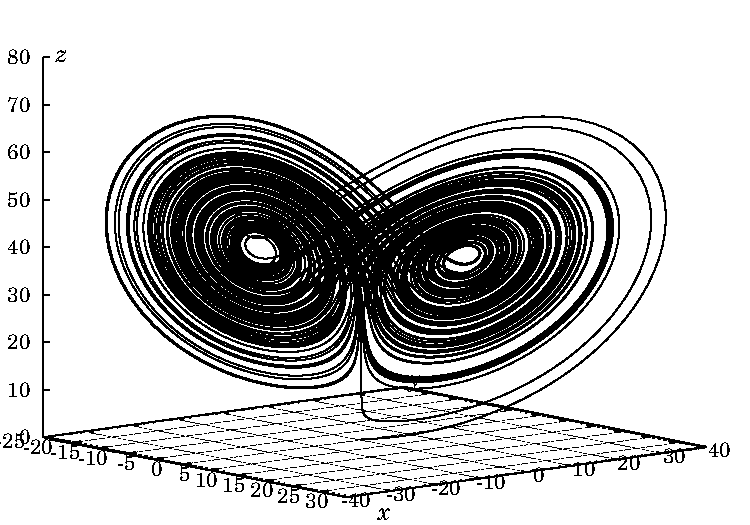
\includegraphics[width=0.5\textwidth]{p/cha/lor_phase3.pdf} }
\caption{Аттрактор системы Лоренца (\ref{atu:eq:lor})}
\label{atu:f:lor_phase}
\end{figure}


 % unfilled, but is near to good


\FloatBarrier

\section{Система Дуффинга} %  % {{{1 _DUFF_
\label{atu:sect:duff}

\LinkRef{
 duff: ASAU-12, 15. APIR-2009. DSMP-2016
  % ~/doc/tex/asau/asau12/atu/atu.tex
  % ~/doc/tex/asau/asau15/atu/atu.tex
}

\subsection{Определение системы и анализ её динамики} %  % {{{2

Рассмотрим нелинейную динамическую систему Дуффинга~\cite{magni_theory_dyn_chaos,atu_asau12}:

\begin{equation}
 \ddot{x} + c_0 \dot{x} + \alpha x + \beta x^3 = u(t) ,
\label{atu:eq:duff}
\end{equation}
%
или её же с сохранением физических размерностей:
%
\begin{equation}
 m \ddot{x} + \nu \dot{x} + k_1 x + k_3 x^3 = F(t) ,
\label{atu:eq:duff_phys}
\end{equation}

Здесь $m$ -- масса объекта,
$x(t)$ -- координата (выходной сигнал),
$u(t) = U_{in} \sin( \omega_{in} t ) $ -- внешняя возмущающая сила,
$ k_1 $ -- коэффициент линейной компоненты возвращающей силы,
$ k_3 $ -- коэффициент при нелинейной части,
$ \alpha $ -- безразмерный коэффициент линейной компоненты возвращающей силы,
 при $ \alpha >0 $ и отсутствии нелинейности определяет собственную частоту: ($\Omega_0^2 = \alpha $),
$ \nu $ и $ c_0$ -- размерный и безразмерный коэффициенты демпфирования,
$ \beta $ -- безразмерный коэффициент нелинейной части.

Идентифицируемый параметр $ \beta $ определяет нелинейные свойства системы.
Следует отметить, что  данная система проявляет хаотические свойства
только при малых значениях параметра \(c_0\). При большем
влиянии диссипативной составляющей система~(\ref{atu:eq:duff}) качественно
не отличается от линейной колебательной системы,
и для её идентификации применимы классические критерии.

% Остальные параметры:
% \(U_{in}=1\), \(\omega_{in}=1\),
% \(c_0 = 0.05\), \( \alpha = -1 \).

На рис.~\ref{atu:f:duff_phase_f_reg} приведены
расширенный фазовый портрет и спектр системы Дуффинга
в режиме сложно-периодических колебаний.
Следует отметить, что существуют условия, при которых добавка к гармоническому входному сигналу
шумоподобной составляющей может перевести систему в хаотический режим~\cite{atu_asau15}.

\begin{figure}[ht!]
\begin{center}
  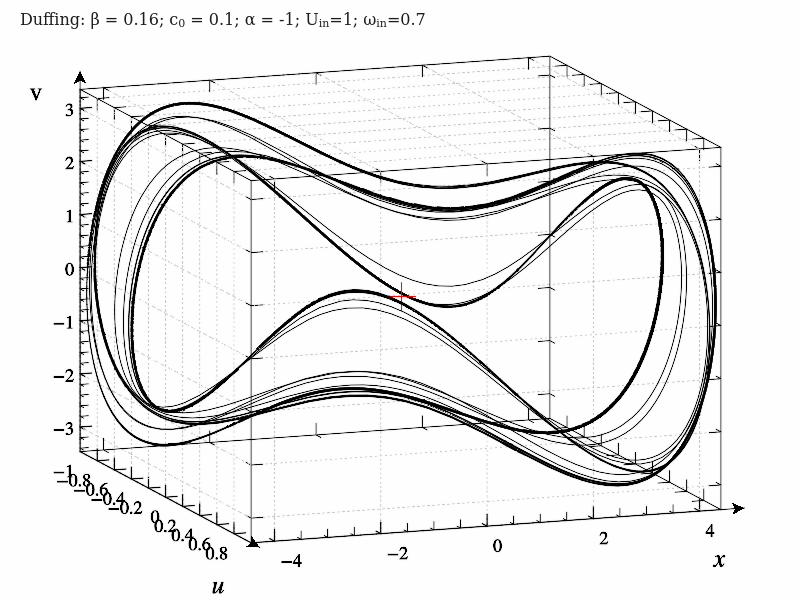
\includegraphics[width=0.49\textwidth]{p/cha/duff/duff_p_1x00_0x70_0x16.png}
  \hfill
  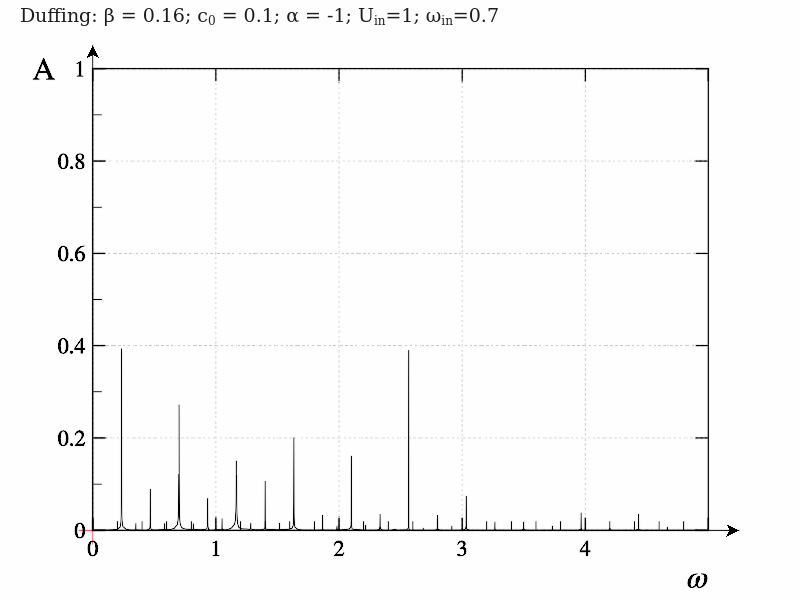
\includegraphics[width=0.49\textwidth]{p/cha/duff/duff_f_1x00_0x70_0x16.png}
\end{center}
  \caption{Расширенный фазовый портрет и спектр системы Дуффинга (\ref{atu:eq:duff}) в режиме сложно-периодических колебаний}
\label{atu:f:duff_phase_f_reg}
\end{figure}

Малые изменения параметра $\beta$ могут перевести систему в режим хаотических
колебаний, при которых вынуждающая частота отображается ярко выраженным пиком
(рис.~\ref{atu:f:duff_phase_f_chaos1}). Также выражены
третья и пятая гармоника входного сигнала,
а участок сплошного спектра выражен слабо.

\begin{figure}[ht!]
\begin{center}
  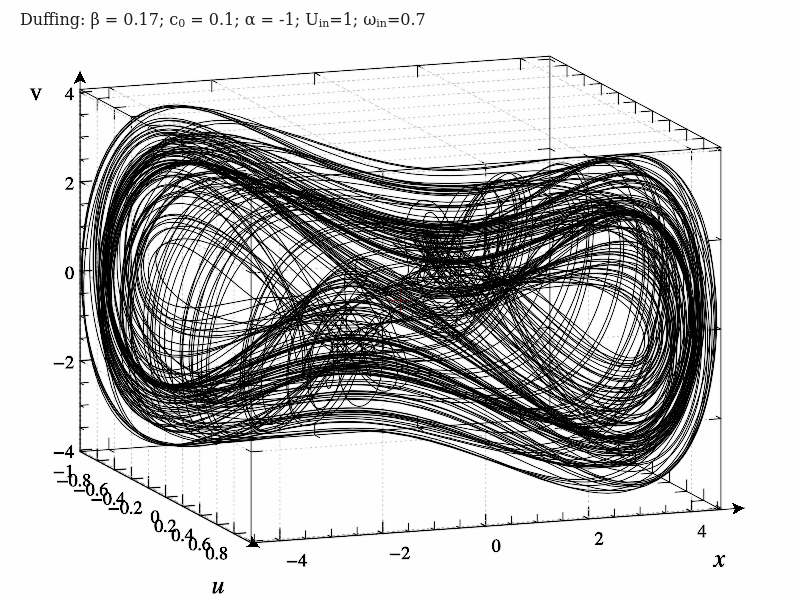
\includegraphics[width=0.49\textwidth]{p/cha/duff/duff_p_1x00_0x70_0x17.png}
  \hfill
  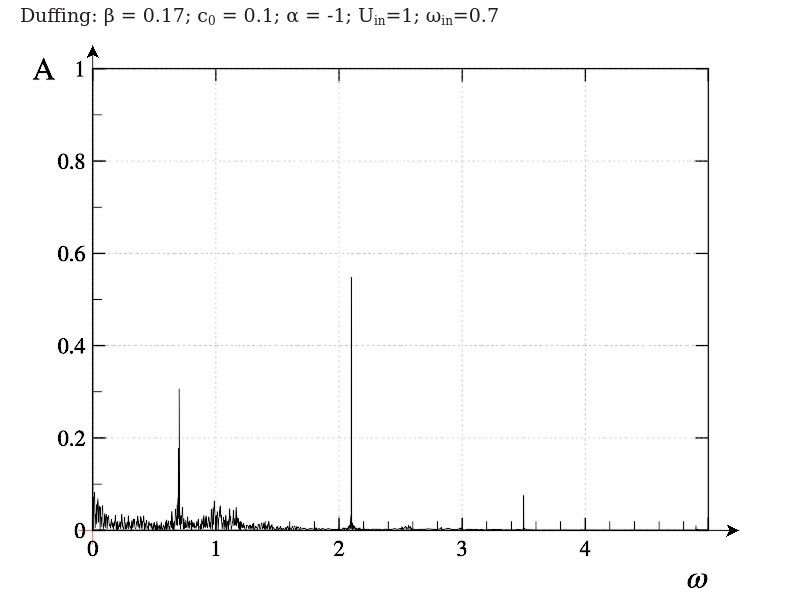
\includegraphics[width=0.49\textwidth]{p/cha/duff/duff_f_1x00_0x70_0x17.png}
\end{center}
  \caption{Расширенный фазовый портрет и спектр системы Дуффинга (\ref{atu:eq:duff}) в режиме слабо выраженных хаотических колебаний}
\label{atu:f:duff_phase_f_chaos1}
\end{figure}


При дальнейшем росте параметра $\beta$ происходит чередование хаотического
и сложно-периодического режимов. Наблюдаются участки,
на которых стабильно наблюдается хаотический режим,
при этом участки сплошного спектра выражены
сильнее~(рис.~\ref{atu:f:duff_phase_f_chaos2}).

\begin{figure}[ht!]
\begin{center}
  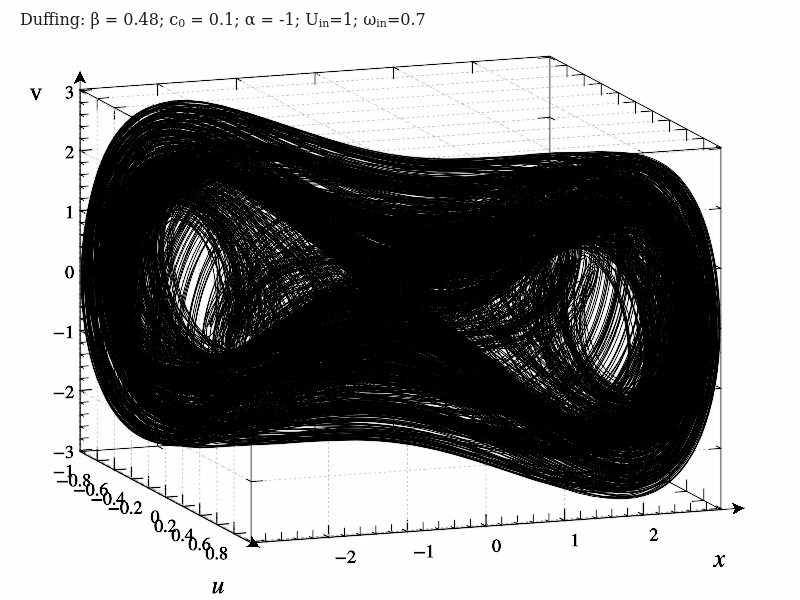
\includegraphics[width=0.49\textwidth]{p/cha/duff/duff_p_1x00_0x70_0x48.png}
  \hfill
  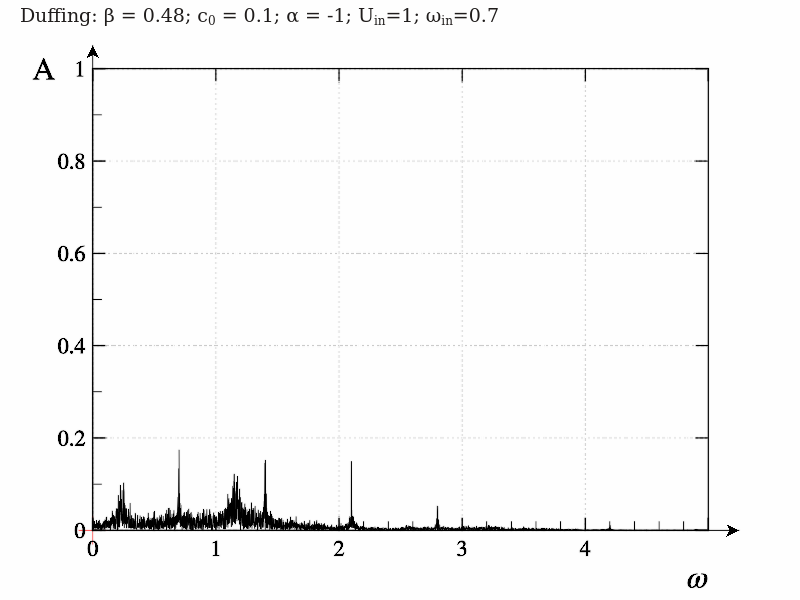
\includegraphics[width=0.49\textwidth]{p/cha/duff/duff_f_1x00_0x70_0x48.png}
\end{center}
  \caption{Расширенный фазовый портрет и спектр системы Дуффинга (\ref{atu:eq:duff}) в режиме выраженных хаотических колебаний}
\label{atu:f:duff_phase_f_chaos2}
\end{figure}

Анализ спектра системы в хаотическом режиме дает
важное наблюдение: участок сплошного спектра
вплотную примыкает к оси ординат. Таким образом
нет такой частоты, ниже которой не наблюдалось собственная
динамика системы, а проявлялись бы только последствия изменения
идентифицируемого параметра. Это к определённым сложностям
при усреднении критериев идентификации.


% \begin{figure}[htb!]
% \centerline{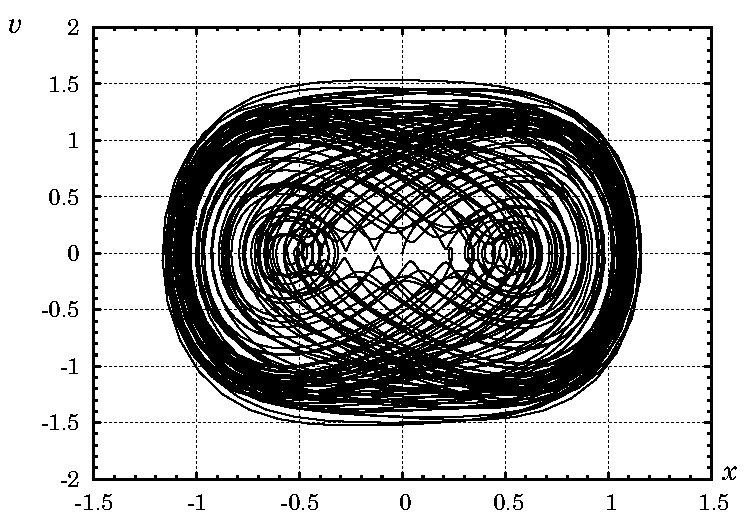
\includegraphics[width=0.5\textwidth]{p/cha/duff_phase.pdf} }
% \caption{Фазовый портрет системы Дуффинга (\ref{atu:eq:duff})}
% \label{atu:f:duff_phase}
% \end{figure}


% }}}2

\subsection{Анализ и выбор критерия}  % {{{2

Рассмотрим возможности определения вида критерия,
основываясь на физических принципах.
Исследуемая система из-за
малой величины \(c_0\) очень близка к консервативной,
и наблюдаемые изменения полной энергии системы
в основном обусловлены взаимодействием с внешним
источником энергии -- входным сигналом \(u(t)\).

Прежде всего отметим, что при неизменных параметрах
системы и входного сигнала, несмотря на то, что
система и её окружение постоянно обмениваются энергией,
среднее значение полной энергии системы остаётся постоянным.
В полную энергию вносят свой вклад кинетическая
%
\begin{equation}
E_k = m \frac{\dot{x}^2(t)}{2}
\label{atu:eq:duff_Ek}
\end{equation}
%
и потенциальная энергия
%
\begin{equation}
E_p = \int\limits_0^x ( k_1 x + k_3 x^3 ) dx =
\frac{k_1 x^2}{2} + \frac{k_3 x^4}{4}.
\label{atu:eq:duff_Ep}
\end{equation}

Как следует из (\ref{atu:eq:duff_Ep}), идентифицируемая
величина \( \beta \)
(в размерном виде ей соответствует параметр \(k_3\))
непосредственно входит только в выражение для
потенциальной энергии, причём её влияние играет большее
значения при максимальных значениях \(x(t)\).
Казалось бы, что в качестве величины, определяющей
критерий идентификации, можно было бы взять
максимальное значение выходного сигнала
при нулевом входе, так как при этом кинетическая энергия системы нулевая,
и создаются благоприятные условия для идентификации.
Однако, это достаточно редкие случаи, чтобы на их основе
строить надёжно работающую систему идентификации, и
естественно, возникает вопрос о точности измерений таких редких
событий.

Воспользуемся тем, что влияние параметра \(\beta\)
наиболее существенно при максимальных значениях \(x\),
и, следовательно, в первую очередь оказывает влияние на величину
%
\begin{equation}
 P = \frac{1}{\tau}\int\limits_0^\tau x^2(t) dt ,
\label{atu:eq:duff_P}
\end{equation}
%
где \(\tau\) -- достаточно большой интервал усреднения.
В свою очередь, данную величину просто измерять,
из-за большого значения \(\tau\) (обычно порядка нескольких десятков
периодов входного сигнала) влияние шумов измерения минимально.

Таким образом, в качестве критерия имеет смысл использовать
$q_{x^2}$, $q_{|x|}$. При этом, ввиду близкой к гиперболической зависимости
имеет смысл включить в рассмотрение и критерий $q_{x^{-2}}$.
Указанные зависимости, полученные при моделировании динамики системы~(\ref{atu:eq:duff})
представлены на рис.~\ref{atu:f:duff_q}.

\begin{figure}[ht!]
\begin{center}
  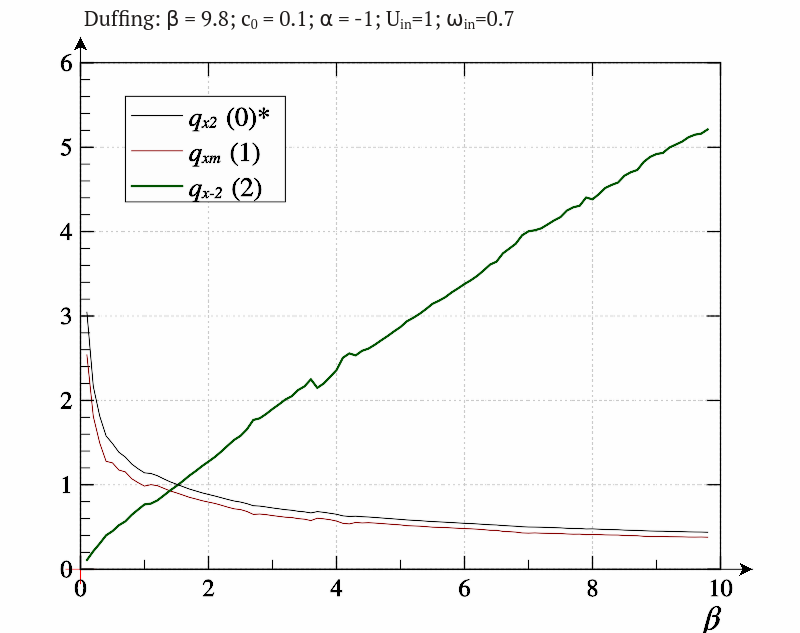
\includegraphics[width=0.49\textwidth]{p/cha/duff/duff_q-p_q_1x00_0x70.png}
\end{center}
  \caption{Зависимости $q_{x^2}(\beta)$, $q_{|x|}(\beta)$,  и $q_{x^{-2}}(\varepsilon) $ для системы Дуффинга}
\label{atu:f:duff_q}
\end{figure}

Анализ графиков позволяет сделать вывод, что критерий $q_{x^{-2}}$
наиболее подходит для проведения идентификации. При это наблюдаются
небольшие нарушения монотонности, что потенциально должно привести к
росту ошибки идентификации в окрестностях этих нарушений.



% }}}2

\subsection{Тестовая задача идентификации для системы Дуффинга}  % {{{2

При синтеза системы идентификации использовалась группа методов ``ql3rlWvnAAW''
при использовании критерия $q_{x^{-2}}$.
Значений параметров выбирались так, что бы обеспечить
наличие всех видов колебаний в рабочем диапазоне:
$U_{in}=1.0$, $\omega_{in}=0.7$, $ \beta \in [1, 4]$.

Рассмотрим процесс идентификации
в квазистационарном случае,
при медленном изменении параметра~(\ref{atu:eq:po_t_ramp}), $p_0=1$, $U_p=2$.
Динамика агентов и различных способов задания $p_\mathrm{id}$
представлена на рис.~\ref{atu:f:duff_id_ramp}.

\begin{figure}[ht!]
\begin{center}
  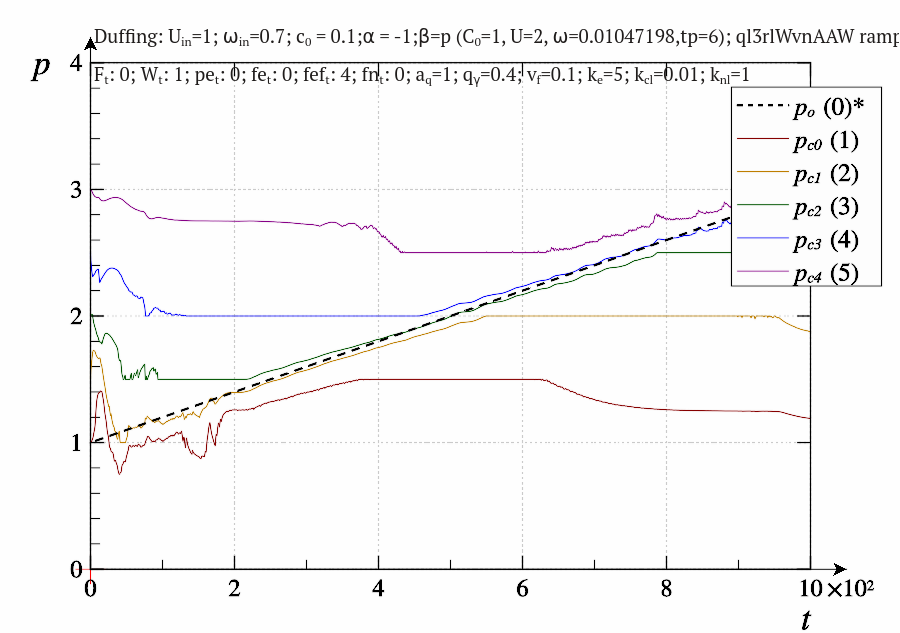
\includegraphics[width=0.49\textwidth]{p/cha/duff/duff_id-p_t_pi_ql3rlWvnAAW_ramp.png}
  \hfill
  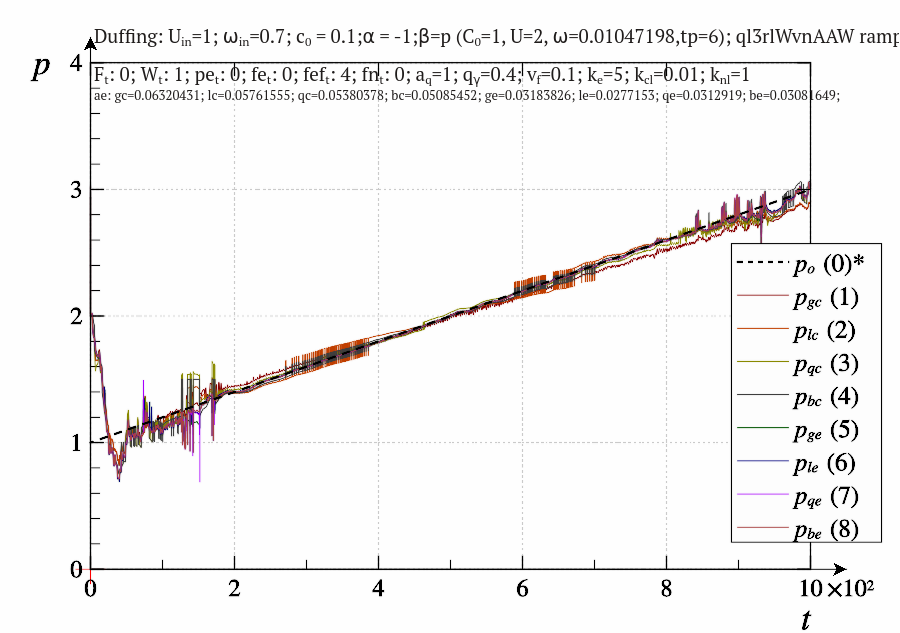
\includegraphics[width=0.49\textwidth]{p/cha/duff/duff_id-p_t_p_ql3rlWvnAAW_ramp.png}
\end{center}
  \caption{Динамика агентов и идентифицируемого значения для системы Дуффинга при условии (\ref{atu:eq:po_t_ramp})}
\label{atu:f:duff_id_ramp}
\end{figure}

Как и для предыдущих систем, метод идентификации демонстрирует свою работоспособность
со всём рабочем диапазоне. Но наблюдаются и существенное
отличие. Особенности спектра системы не дают возможности построить достаточно эффективный
фильтр. Как следствие, у значений $p_\mathrm{id}$ наблюдаются
высокочастотные колебания. Наиболее подвержены этому явлению
методы координаторов $p_{lc}$ и $p_{bc}$.

Рассмотрим реакцию системы идентификации на скачкообразные
изменения параметра, динамика которого была задана (\ref{atu:eq:po_t_sign}),
$p_0=2$, $U_p=0.8$, $\omega_{in}=0.01047$.
Результаты представлены на рис.~\ref{atu:f:duff_id_sign}.

\begin{figure}[ht!]
\begin{center}
  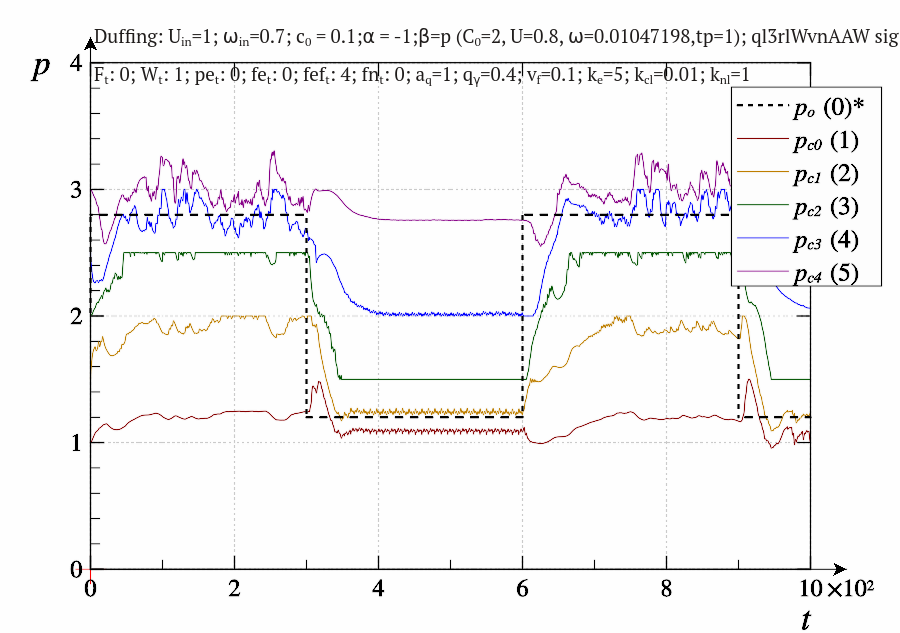
\includegraphics[width=0.49\textwidth]{p/cha/duff/duff_id-p_t_pi_ql3rlWvnAAW_sign.png}
  \hfill
  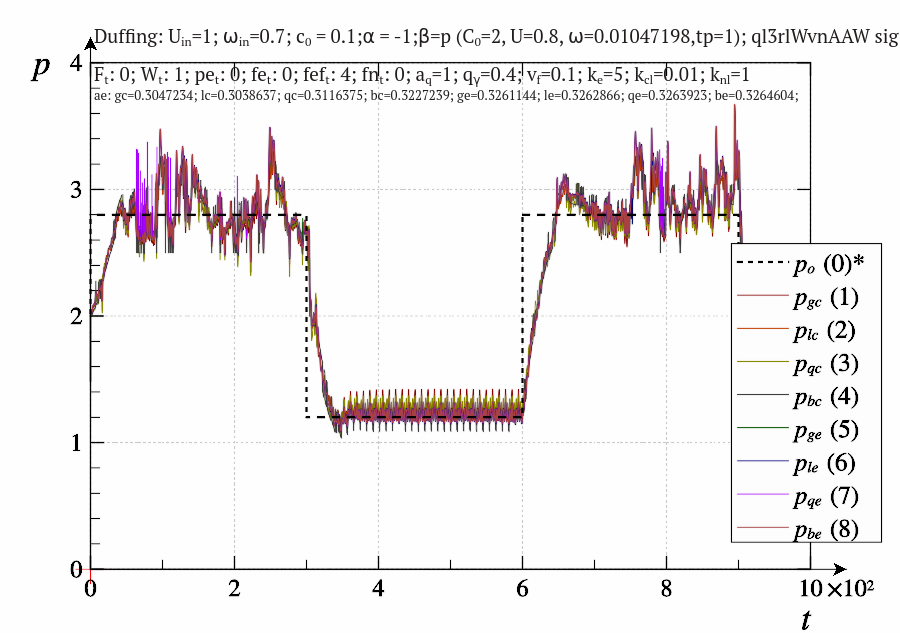
\includegraphics[width=0.49\textwidth]{p/cha/duff/duff_id-p_t_p_ql3rlWvnAAW_sign.png}
\end{center}
  \caption{Динамика агентов и идентифицируемого значения для системы Дуффинга при условии (\ref{atu:eq:po_t_sign})}
\label{atu:f:duff_id_sign}
\end{figure}

Помимо уже отмеченной особенности, заключающейся в повышенном уровне колебаний,
обращает на себя факт увеличения ошибки идентификации при $\beta \approx 3$.
В этой области значений параметра наблюдается устойчивый хаотический режим,
с сплошным спектром вплоть но нулевой частоты.

При более плавной динамике параметра
(\ref{atu:eq:po_t_sin}),
$p_0=2$, $U_p=0.8$, $\omega_{in}=0.01047$
наблюдается аналогичная картина
(рис.~\ref{atu:f:duff_id_sign}),
но размах колебаний существенно меньше.

\begin{figure}[ht!]
\begin{center}
  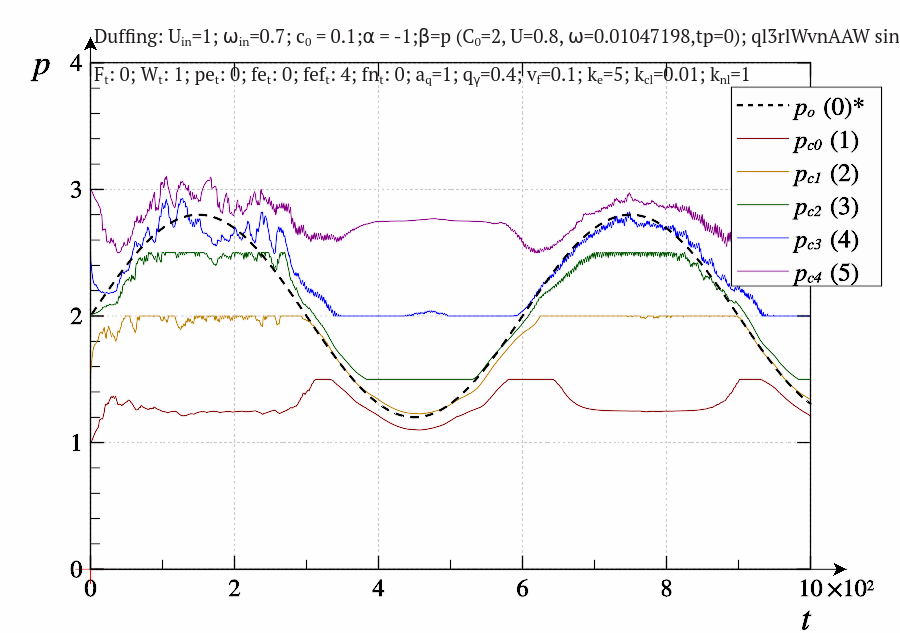
\includegraphics[width=0.49\textwidth]{p/cha/duff/duff_id-p_t_pi_ql3rlWvnAAW_sin.png}
  \hfill
  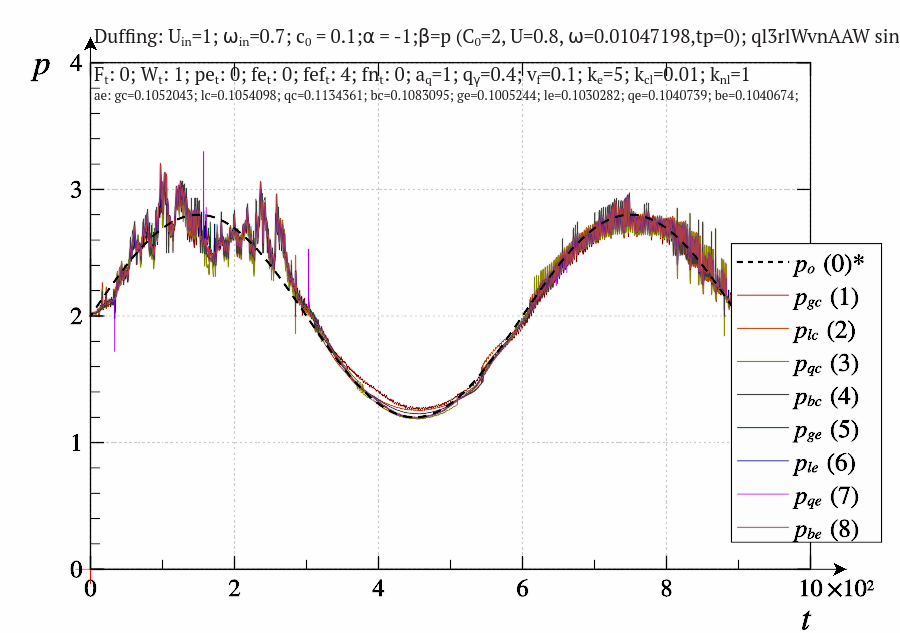
\includegraphics[width=0.49\textwidth]{p/cha/duff/duff_id-p_t_p_ql3rlWvnAAW_sin.png}
\end{center}
  \caption{Динамика агентов и идентифицируемого значения для системы Дуффинга при условии (\ref{atu:eq:po_t_sin})}
\label{atu:f:duff_id_sin}
\end{figure}


% }}}2

\subsection{Влияние параметров системы идентификации на ошибку идентификации для системы Дуффинга}  % {{{2

Эти зависимости представлены на рис.~\ref{atu:f:duff_e_a_q}.

\begin{figure}[ht!]
\begin{center}
  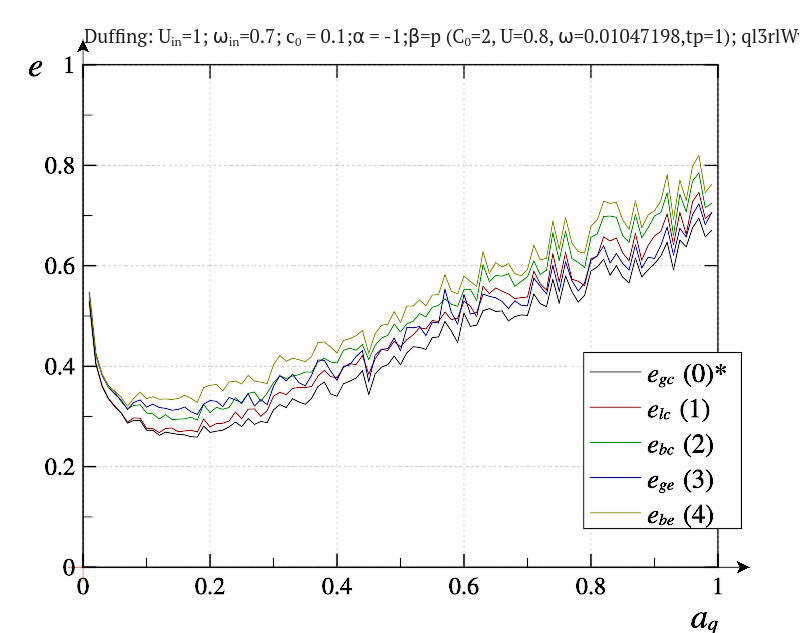
\includegraphics[width=0.49\textwidth]{p/cha/duff/duff_id-p_a_q_sign.png}
  \hfill
  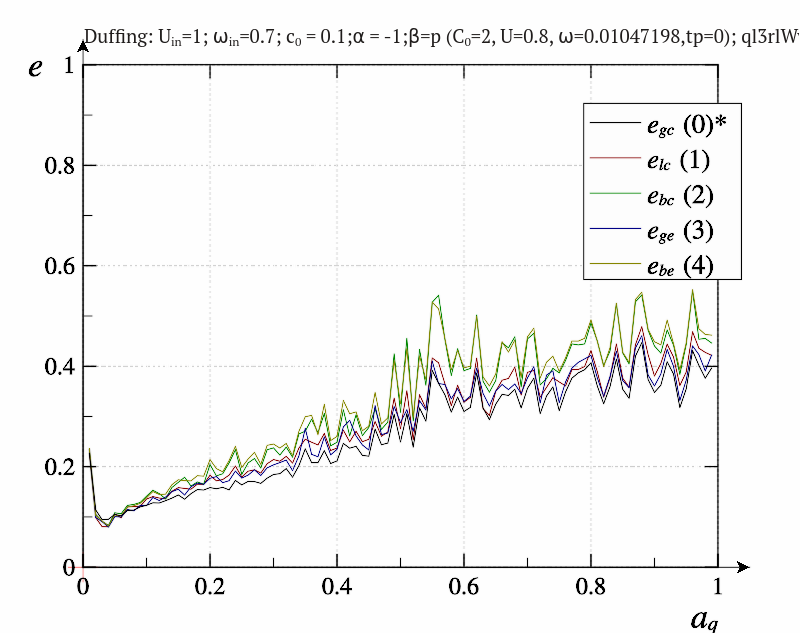
\includegraphics[width=0.49\textwidth]{p/cha/duff/duff_id-p_a_q_sin.png}
\end{center}
  \caption{Зависимости $\bar{e}(a_q)$ для системы Дуффинга}
\label{atu:f:duff_e_a_q}
\end{figure}


\begin{figure}[ht!]
\begin{center}
  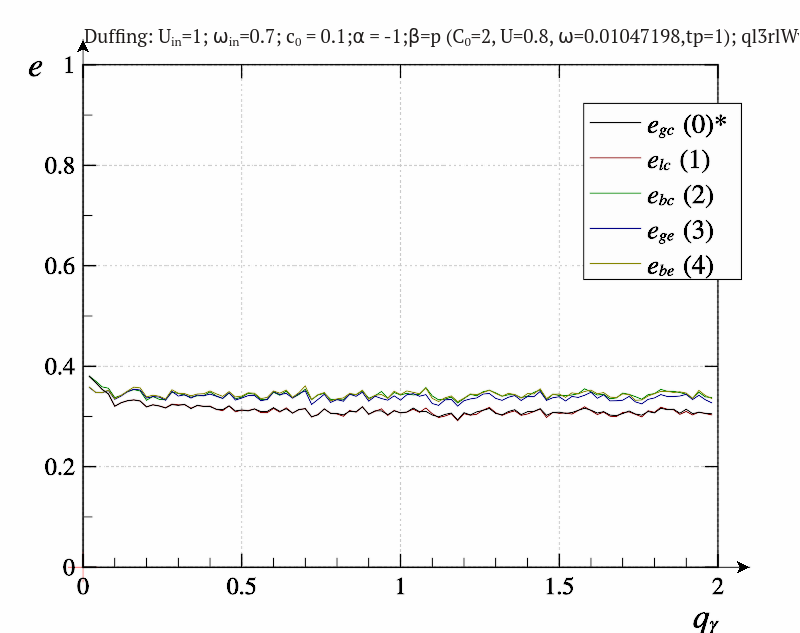
\includegraphics[width=0.49\textwidth]{p/cha/duff/duff_id-p_q_gamma_sign.png}
  \hfill
  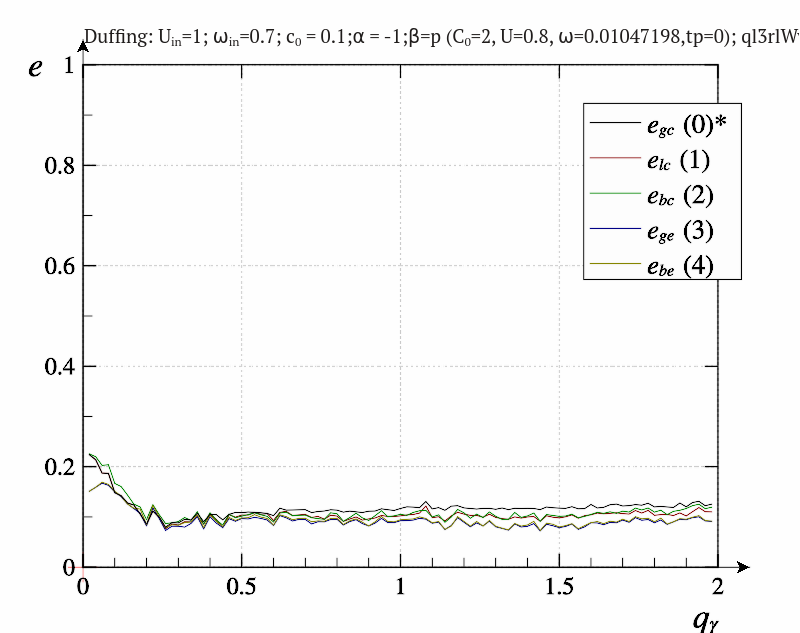
\includegraphics[width=0.49\textwidth]{p/cha/duff/duff_id-p_q_gamma_sin.png}
\end{center}
  \caption{Зависимости $\bar{e}(q_\gamma)$ для системы Дуффинга}
\label{atu:f:duff_e_q_gamma}
\end{figure}

\begin{figure}[ht!]
\begin{center}
  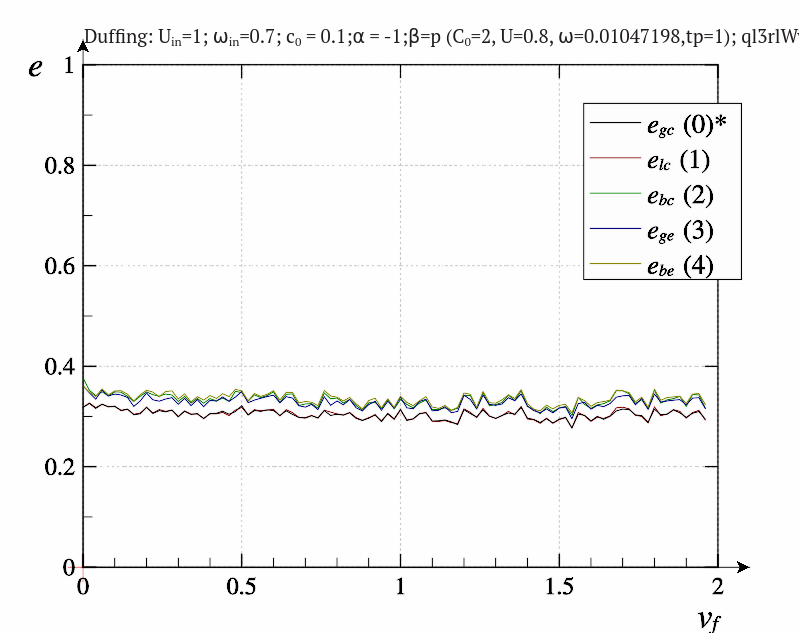
\includegraphics[width=0.49\textwidth]{p/cha/duff/duff_id-p_v_f_sign.png}
  \hfill
  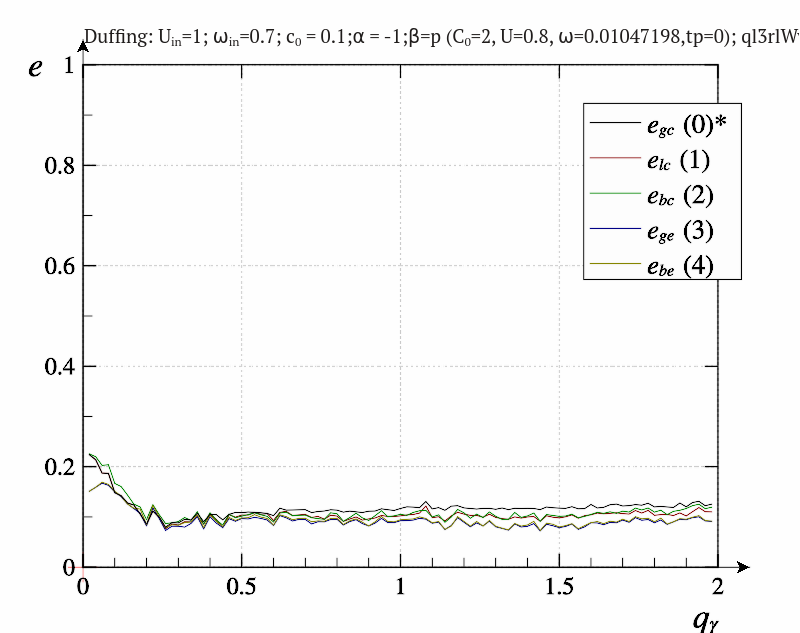
\includegraphics[width=0.49\textwidth]{p/cha/duff/duff_id-p_q_gamma_sin.png}
\end{center}
  \caption{Зависимости $\bar{e}(v_f)$ для системы Дуффинга}
\label{atu:f:duff_e_v_f}
\end{figure}

\begin{figure}[ht!]
\begin{center}
  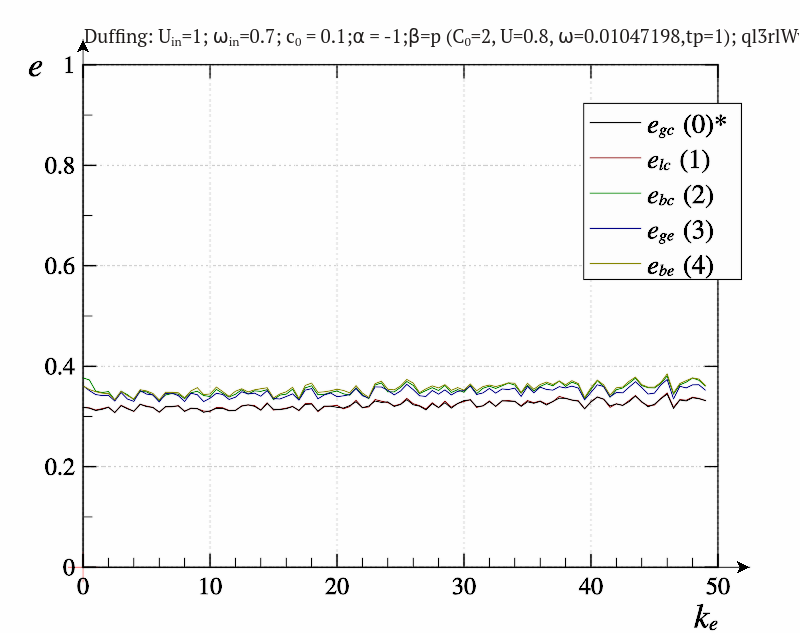
\includegraphics[width=0.49\textwidth]{p/cha/duff/duff_id-p_k_e_sign.png}
  \hfill
  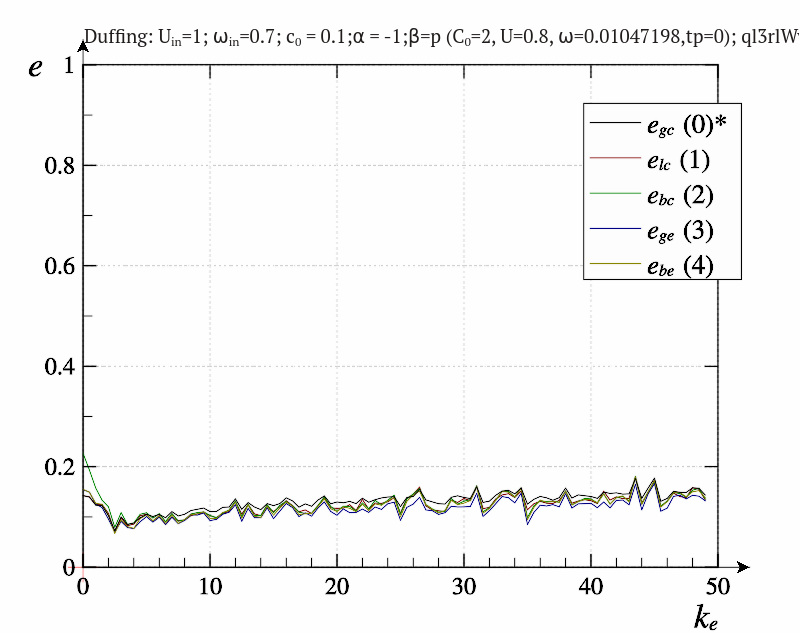
\includegraphics[width=0.49\textwidth]{p/cha/duff/duff_id-p_k_e_sin.png}
\end{center}
  \caption{Зависимости $\bar{e}(k_e)$ для системы Дуффинга}
\label{atu:f:duff_e_k_e}
\end{figure}

\begin{figure}[ht!]
\begin{center}
  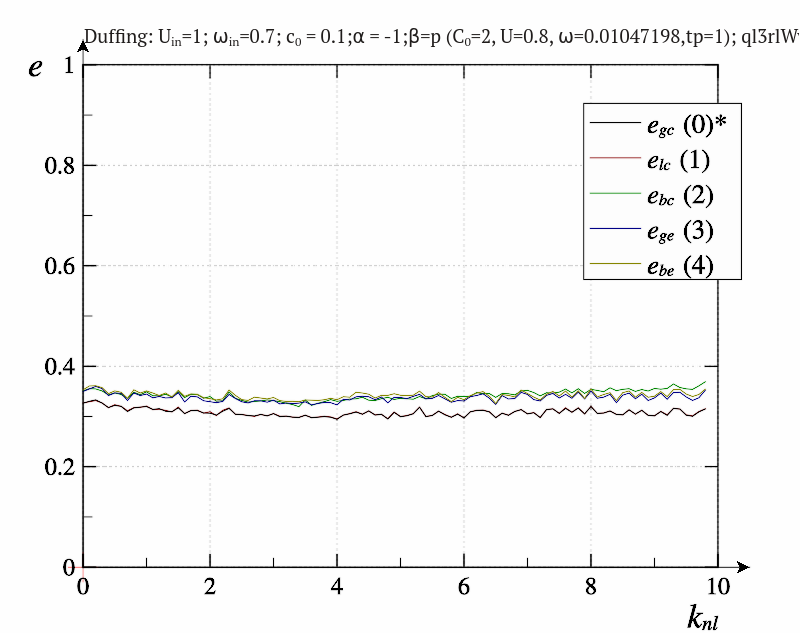
\includegraphics[width=0.49\textwidth]{p/cha/duff/duff_id-p_k_nl_sign.png}
  \hfill
  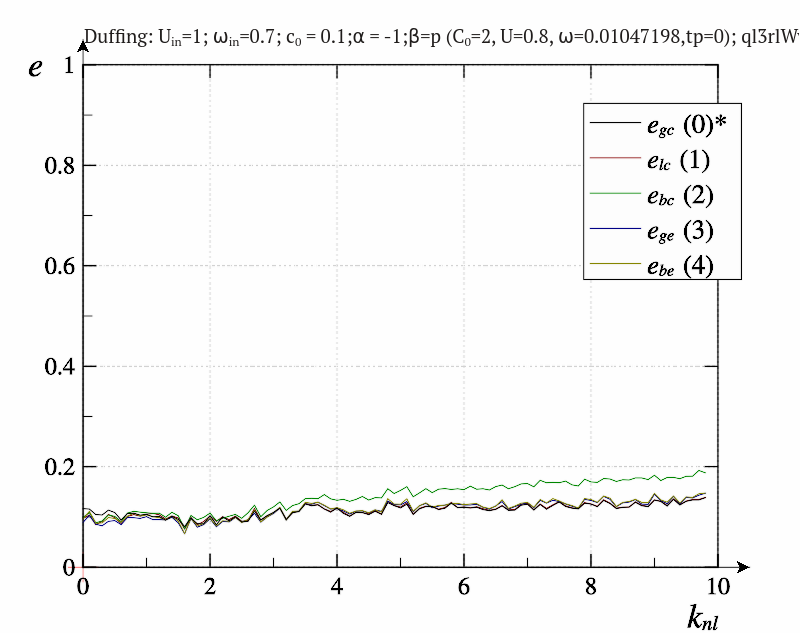
\includegraphics[width=0.49\textwidth]{p/cha/duff/duff_id-p_k_nl_sin.png}
\end{center}
  \caption{Зависимости $\bar{e}(k_{nl})$ для системы Дуффинга}
\label{atu:f:duff_e_k_nl}
\end{figure}

\begin{figure}[ht!]
\begin{center}
  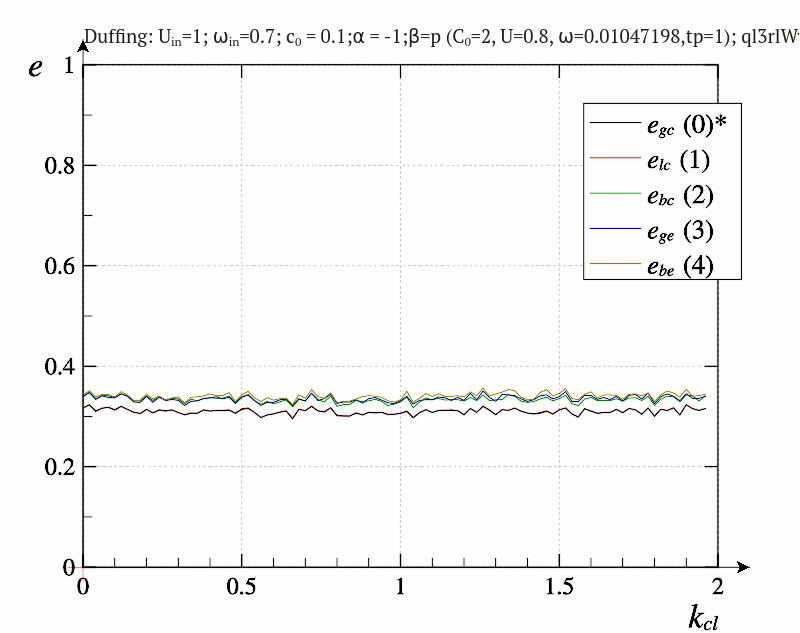
\includegraphics[width=0.49\textwidth]{p/cha/duff/duff_id-p_k_cl_sign.png}
  \hfill
  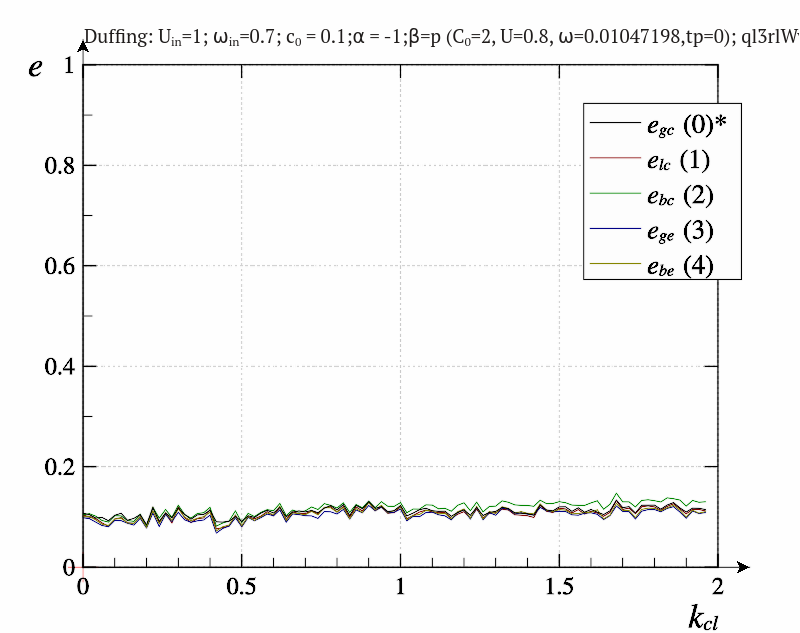
\includegraphics[width=0.49\textwidth]{p/cha/duff/duff_id-p_k_cl_sin.png}
\end{center}
  \caption{Зависимости $\bar{e}(k_{cl})$ для системы Дуффинга}
\label{atu:f:duff_e_k_cl}
\end{figure}


% }}}2

\subsection{Выводы}  % {{{2

Выводы

% }}}2

% }}}1

% vim: fdm=marker foldlevel=1 foldignore="%#" fdc=4 ft=tex



\FloatBarrier

\section{Система Чуа} %% {{{1 _CHUA_
\label{atu:sect:chua}

\LinkRef{
 chua: ASAU-18, MKMM-2014, APIR-2011
}

\subsection{Визначення системи та аналіз її динаміки} % {{{2 _chua_task

Однією з відомих хаотичних систем, легко реалізованих як аналітично,
(\ref{atu:eq:chua}), так і схемотехнічно (рис.~\ref{atu:f:chuascheme}),
є нелінійна система Чуа~\cite{moon_chaotic_vibr,buga_chua,Kennedy92robustop,Kennedy_Chua_primer}:

\begin{figure}[htb!]
\begin{center}
% vi:syntax=tex

\begin{circuitikz}[line width=0.7]
  \ctikzset{bipoles/thickness=2}
  \def\Top{3.0}
  \draw (0.0,0.0) to[L,l=$L$,i=$I_L$] (0,\Top)
   to[R=R] (6.0,\Top)
   to[ageneric,l=$R_c$] (6.0,0.0) -- (0.0,0.0);
  \draw(1.5,0.0) to[C,l=$C_2$,v=$V_2$] (1.5,\Top );
  \draw(4.5,0.0) to[C,l=$C_1$,v=$V_1$] (4.5,\Top );
\end{circuitikz}

% \begin{tikzpicture}[circuit ee IEC,very thick,circuit symbol unit=3.5mm]
%   \node (L1) at (0,1.5) [point up,elelem,inductor={info = $L$}] {};
%   \node      at (0.2,2.4) {$I_L$};
%   \node (C2) at (1.5,1.5) [point up,elelem,capacitor={info = $C_2$}] {};
%   \node      at (1.8,1.8) {$V_2$};
%   \node (pc2d) at (1.5,0) [contact] {};
%   \node (pc2u) at (1.5,3) [contact] {};
%   \node (C1) at (5.0,1.5) [point up,elelem,capacitor={info = $C_1$}] {};
%   \node      at (5.3,1.8) {$V_1$};
%   \node (pc1d) at (5,0) [contact] {};
%   \node (pc1u) at (5,3) [contact] {};
%   \node (R) at (3,3) [elelem,resistor={info = $R$}] {};
%   \node (Rc) at (7,1.5) [elelem,point up,resistor={info = $R_c$}] {};
%   \draw (Rc) ++(-0.15,-0.7) rectangle+(0.3,0.2);
%   \draw (L1) |- (pc2d) -- (pc1d) -| (Rc) [wire];
%   \draw (L1) |- (pc2u) -- (R) -- (pc1u) -| (Rc) [wire];
%   \draw (pc2u) -- (C2) [wire]; \draw (pc2d) -- (C2) [wire];
%   \draw (pc1u) -- (C1) [wire]; \draw (pc1d) -- (C1) [wire];
%   \node (Gr) at (5,-0.3) [elelem,point down,ground] {};
%   \draw (pc1d) -- (Gr) [wire];
% \end{tikzpicture}

\end{center}
\caption{Умовна електричний ланцюг, що реалізує хаотичну систему Чуа}
\label{atu:f:chuascheme}
\end{figure}


\begin{equation}
\begin{cases}
  C_1 \dot{V_1}  = \frac{1}{R} ( V_2 - V_1 ) - g(V_1), \\
  C_2 \dot{V_2}  = \frac{1}{R} ( V_1 - V_2 ) + I_L, \\
  \dot{I_L}      = - \frac{1}{L} V_2 .
\end{cases}
\label{atu:eq:chua}
\end{equation}

Єдиним нелінійним елементом в цій системі є ``діод Чуа''
(позначений на схемі як $R_c$) з
характеристикою
$g(V)$~(рис.~\ref{atu:f:diodchua}),
характеризується різними від'ємними нахилами ($m_0 $ і $ m_1 $)
на різних ділянках, і тим самим виступає у ролі керованого джерела енергії.
%
\begin{equation}
g(V) =
\begin{cases}
  m_1 V = ( m_0 + m_2 ) V , & |V| <   U_0, \\
  m_0 V ,                   & |V| \ge U_0.
\end{cases}
\label{atu:eq:diodchua}
\end{equation}

\begin{figure}[htb!]
\begin{center}
% vi:syntax=tex
\begin{tikzpicture}
  \coordinate (XMIN) at (-4.5,0.0);
  \coordinate (XMAX) at ( 4.5,0.0);
  \coordinate (YMIN) at (0,-2.5);
  \coordinate (YMAX) at (0, 2.5);
  \draw (XMIN) -- (XMAX) [medline,->] node[below] {$U$};
  \draw (YMIN) -- (YMAX) [medline,->] node[left]  {$I$};
  \draw (-4,2) -- (-1,1) -- (1,-1) -- (4,-2) [boldline];
  \draw (1,-1) -- (1,0) [dashed,medline];
  \draw (1,-1) -- (4,-1) [dashed,medline];
  \draw (1.41,0) arc [medline,->,start angle=0,end angle=-45,radius=1.41];
  \draw (1,-1) ++(2,0) arc [medline,->,start angle=0,end angle=-18,radius=2.0];
  \filldraw (1,0) circle[radius=0.05,fill=black] node[above] {$U_0$};
  \node[right] at (1.2,-0.6) {$\alpha_1: \tan(\alpha_1)=m_1$};
  \node[right] at (3.0,-1.3) {$\alpha_0$};
\end{tikzpicture}

\end{center}
\caption{Характеристика \(I = g (V) \) діода Чуа}
\label{atu:f:diodchua}
\end{figure}


При цьому параметр \(m_0\) визначає надходження енергії в
систему при великих амплітудах \(V_1\), і, в цілому, характеризує
енергетичні можливості джерела. Аналогічно, параметр \(m_1\)
характеризує надходження енергії при малих коливаннях, зокрема,
визначає, чи буде система переходити в коливальний стан при
малих початкових збурень, і якою буде режим цих коливань. З
іншого боку, оскільки параметр \(m_1\) є сумою ``глобального
параметра'' \(m_0 \) і ``доважку'', що визначає додатковий внесок
при малих амплітудах, то має сенс перейти від параметра \(m_1 \) до
параметру \(m_2 = m_1 - m_0 \), який і визначає в цілому нелінійність
системи. При \(m_2 = 0 \) система стає лінійною і не представляє
особливого інтересу.
У даній роботі як параметр, що підлягає ідентифікації, обрано саме~$m_2$.

Відомо, що в залежності від величини параметра
$ m_2 $, система може переходити в режими загасання, періодичного
і складно-періодичного руху, а також в режим хаотичних
коливань~\cite{anisch_nonlin_eff,magni_new_meth,Chua_double_scroll}. При цьому
складно-періодичний і хаотичний рух чергуються зі зміною
величини \(m_2\).


Класично параметри системи Чуа задаються наступним чином~\cite{buga_chua}:
$C_1 = 1/9$, $C_2 = 1$, $L= 1/7$, $R = 1/0.7$, $m_0=-0.5$, $ m_2 \in [ -0.15; -0.7 ] $.

Введемо позначення:
\[
  a_{11} = \frac{1}{R C_1}; \;
  a_{13} = \frac{1}{C_1}; \;
  a_{21} = \frac{1}{R C_2}; \;
  a_{23} = \frac{1}{C_2}; \;
  a_{31} = -\frac{1}{L}; \;
  a_g = - \frac{m_0}{C_1}; \;
  \mu = - \frac{m_2}{C_1}.
\]
%
%\noindent
Тоді:
%
\begin{equation}
\begin{cases}
  \dot{V}_1  = -a_{11} V_1 + a_{11}  V_2  + g_1(V_1) , \\
  \dot{V}_2  = +a_{21} V_1 - a_{21}  V_2  + a_{23} I_L    , \\
  \dot{I}_L  =  a_{31} V_2.
\end{cases}
\label{atu:eq:chua2}
\end{equation}
%
%
\begin{equation}
g_1(V) =
\begin{cases}
  ( a_g + \mu ) V , & |V| <   U_0, \\
  a_g V           , & |V| \ge U_0.
\end{cases}
\label{atu:eq:diodchua2}
\end{equation}

При цьому перелічені класичні значення параметрів будуть представлені таким чином:
$ a_{11} = 6.5 $, $a_{21} = 0.7$, $ a_{23} = -7 $, $ a_g = 4.5 $,
$ \mu \in [ 1.29 ; 5.6 ] $.
Відповідно, в цих позначеннях ідентифікований параметр є~$\mu$. Він задає вид динаміки системи.


\begin{figure}[htb!]
  \PicDouble{p/cha/chua/chua_1-p_xyz_mu=2x74.png}{p/cha/chua/chua_1-p_xyz_mu=4x50.png}
  \caption{Аттрактор системи Чуа (\ref{atu:eq:chua2}) при різних значеннях $\mu$: 2.74~(a) і 4.5~(b)}
  \label{atu:f:chua_phase}
\end{figure}


% }}}2

\subsection{Аналіз і вибір критеріїв}%{{{2


Для визначення виду критерію розглянемо залежності
$q_{*}(\mu)$ (індексом ``*'' будемо позначати застосування будь-якого
з індексів, що позначають вихідний сигнал для критерію і спосіб
усереднення), отримані шляхом моделювання для системи Чуа (рис.~\ref{atu:f:chua_q}):

\begin{figure}[htb!]
  \PicDouble{p/cha/chua/chua_q-p_mu2.png}{p/cha/chua/chua_q-p_mu1.png}
  \caption{Залежності $q_{*}(\mu) $ для системи Чуа (\ref{atu:eq:chua2})}
\label{atu:f:chua_q}
\end{figure}

З аналізу графіків зроблено висновок, що величина $q_{V_1}(\mu)$
є найкращим кандидатом в критерії, з огляду на близьку до
лінійної залежності в робочому діапазоні~\cite{atu_apir2011}.

Наступним важливим параметром, необхідним для ефективної
роботи системи ідентифікації, є характерний час оцінювання
$\tau$ (\ref{atu:eq:qlin}), або ж зворотна йому величина
$a_q$.

Для попереднього оцінювання величини
$a_q$ розглянемо спектри системи при різних
$\mu$ (рис.~\ref{atu:f:chua_spectrum}). Як випливає з графіків, спектр системи
досить обмежений зверху, проте, в хаотичному режимі є суцільним
практично до нуля. Це не дає можливості безпосередньо визначити
$ a_q $ виходячи із спектру, однак, перші суттєві піки
спостерігаються при
$\omega \approx 0.3 $, отже, первинне значення
$a_q $ можна оцінити як
$a_q \approx 0.3 / \pi \approx 0.1 $ .


\begin{figure}[htb!]
  \PicTriple{p/cha/chua/chua_f-p_f_mu=2x00.png}{p/cha/chua/chua_f-p_f_mu=2x74.png}{p/cha/chua/chua_f-p_f_mu=4x50.png}
  \caption{Спектри системи Чуа (\ref{atu:eq:chua2}) при різних значеннях $\mu$: 2.0~(a), 2.74~(b), 4.5~(c)}
  \label{atu:f:chua_spectrum}
\end{figure}

Наступний спосіб оцінити
$a_q $ --- дослідити отриману в результаті моделювання залежність
середньоквадратичного відхилення
$e_q $ оцінки величини
$q$, нормованої на саму величину
$q$ в стаціонарному випадку. Отримана залежність представлена
на рис.~\ref{atu:f:chua_tau}.

\begin{figure}[htb!]
\begin{center}
  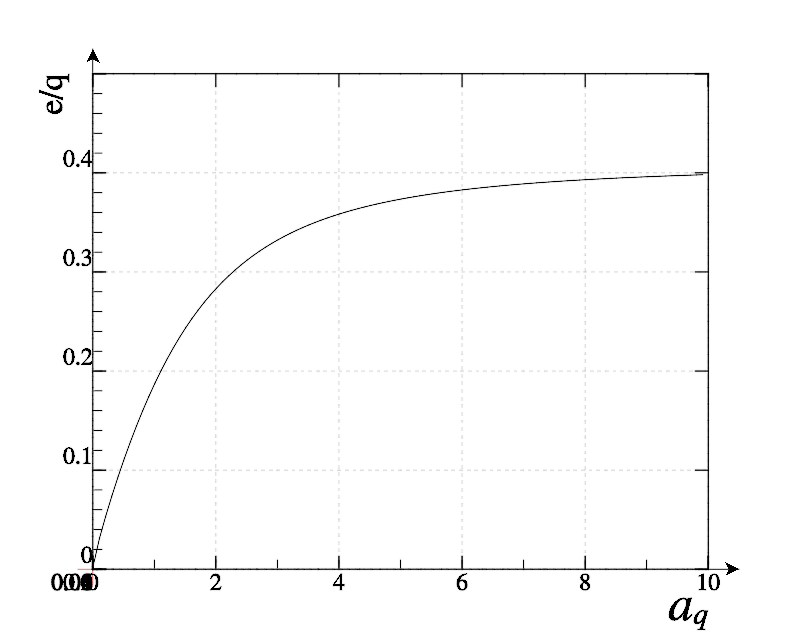
\includegraphics[width=0.4\textwidth]{p/cha/chua/chua_tau-p_e_a.png}
\end{center}
\caption{Типова залежність $ e_q / q (a_q) $ для системи (\ref{atu:eq:chua2})}
\label{atu:f:chua_tau}
\end{figure}

З цього графіка можна зробити висновок, що первісна оцінка $a_q$ була зроблена коректно.

% }}}2

\subsection{Тестова задача ідентифікації для системи Чуа}%{{{2

Відповідно до отриманих даних, і використовуючи
пропозиції~(\ref{atu:eq:po_t_sign}) і~(\ref{atu:eq:po_t_sin}), визначимо тестове
завдання наступним чином:
%
\begin{equation}
 \mu_o(t) = p_0 + U_p \sign \sin( \omega_p t )
  \label{atu:eq:chua_mu_sign}
\end{equation}
%
\begin{equation}
 \mu_o(t) = p_0 + U_p \sin( \omega_p t ).
  \label{atu:eq:chua_mu_sin}
\end{equation}
%
де:
$p_0 = 3.25$, $U_p=0.6$, $\omega_p = \pi / 300$.

При моделюванні процесів ідентифікації було виявлено наступне
явище: якщо динаміка параметра
$ \mu $ задана (\ref{atu:eq:chua_mu_sign}), то існують такі значення
$ p_0 $ і $ U_p $, при яких система повністю втрачає стійкість. Для
схемотехнічних реалізацій системи Чуа таких явищ не
спостерігається, так як реальні системи мають обмежені
можливості з підтримки від'ємного опору. Для таких
випадків подання діода Чуа у вигляді (\ref{atu:eq:diodchua}) не є
адекватним~\cite{atu_kher2014}. Точніше, з огляду на той факт, що
схемотехнічні реалізації з'явилися після аналітичного
дослідження, більш правильним буде твердження про те, що реалізації
недостатньо адекватно реалізують аналітичну залежність
для діода Чуа. Більш адекватна реалізація вимагає наявності
необмеженого джерела енергії. З урахуванням вищезазначеного,
множина тестових систем для даної задачі є більш обмеженою.

На рис.~\ref{atu:f:chua_id_ql3rlWvnAAW_sign} представлені результати
моделювання процесу ідентифікації групою методів ql3rlWvnAAW за
умови~(\ref{atu:eq:chua_mu_sign}).

\begin{figure}[htb!]
  \PicDouble{p/cha/chua/ql3rlWvnAAW/chua_id-p_t_pi_ql3rlWvnAAW_sign.png}{p/cha/chua/ql3rlWvnAAW/chua_id-p_t_p_ql3rlWvnAAW_sign.png}
  \caption{Процес ідентифікації параметра ``$\mu$'' системи Чуа групою методів ql3rlWvnAAW за умови~(\ref{atu:eq:chua_mu_sign}): динаміка агентів~(a) та $p_\mathrm{id}$~(b)}
  \label{atu:f:chua_id_ql3rlWvnAAW_sign}
\end{figure}

При заданих умовах система цілком працездатна, рівень коливань
ідентифікованого параметра цілком відповідає задачі.

На рис.~\ref{atu:f:chua_id_ql3rlWvnAAW_sin} представлені результати
моделювання процесу ідентифікації групою методів ql3rlWvnAAW за
умови~(\ref{atu:eq:chua_mu_sin}).

\begin{figure}[htb!]
  \PicDouble{p/cha/chua/ql3rlWvnAAW/chua_id-p_t_pi_ql3rlWvnAAW_sin.png}{p/cha/chua/ql3rlWvnAAW/chua_id-p_t_p_ql3rlWvnAAW_sin.png}
  \caption{Процес ідентифікації параметра ``$\mu$'' системи Чуа групою методів ql3rlWvnAAW за умови~(\ref{atu:eq:chua_mu_sin}): динаміка агентів~(a) та $p_\mathrm{id}$~(b)}
\label{atu:f:chua_id_ql3rlWvnAAW_sin}
\end{figure}

Як загальний рівень похибки, так і розмах коливань значення
параметра в цьому випадку помітно менше, аналогічно процесам
ідентифікації інших розглянутих хаотичних систем.

Процес ідентифікації в умовах, коли параметр
$ \mu $ повільно і лінійно ``пробігає'' увесь робочий
діапазон, що підлягає аналізу, проілюстрований на рис.~\ref{atu:f:chua_id_ql3rlWvnAAW_ramp}.

\begin{figure}[htb!]
  \PicDouble{p/cha/chua/ql3rlWvnAAW/chua_id-p_t_pi_ql3rlWvnAAW_ramp.png}{p/cha/chua/ql3rlWvnAAW/chua_id-p_t_p_ql3rlWvnAAW_ramp.png}
  \caption{Процес ідентифікації параметра ``$\mu$'' системи Чуа групою методів ql3rlWvnAAW за умови~(\ref{atu:eq:po_t_ramp}): динаміка агентів~(a) та $p_\mathrm{id}$~(b)}
\label{atu:f:chua_id_ql3rlWvnAAW_ramp}
\end{figure}

Залежності на графіках свідчать про те, що з урахуванням рівня
похибки, ідентифікація на всьому діапазоні відбувається без
будь-яких істотних порушень.


% }}}2


\subsection{Вплив параметрів системи ідентифікації на похибку ідентифікації для системи Чуа} % {{{2

Для більш точного налаштування параметрів самої системи
ідентифікації розглянемо залежності помилок ідентифікації
від основних параметрів системи ідентифікації.

Для перевірки коректності вибору величини
$a_q$ були побудовані залежності помилок ідентифікації
(рис.~\ref{atu:f:chua_e_a_q}) від цього параметра.


\begin{figure}[htb!]
  \PicDouble{p/cha/chua/ql3rlWvnAAW/chua_id-p_a_q_sign.png}{p/cha/chua/ql3rlWvnAAW/chua_id-p_a_q_sin.png}
  \caption{Залежності $\overline{e}(a_q) $ для системи (\ref{atu:eq:chua2}) при умовах (\ref{atu:eq:chua_mu_sign})~(a) і (\ref{atu:eq:chua_mu_sin})~(b)}
  \label{atu:f:chua_e_a_q}
\end{figure}

Як видно з результатів моделювання, первісна оцінка ``коректного'' значення величини
$a_q$ була зроблена досить точно. При цьому, при синусоїдальній
зміні параметра об'єкта менша похибка ідентифікації
спостерігається при менших значеннях
$a_q$, що пов'язано з тим, в даному випадку немає необхідності в
стеженні за параметром, величина якого стрибкоподібно змінюється,
і, отже, припустим більший час оцінювання. Навпаки, в разі
(\ref{atu:eq:chua_mu_sign}) збільшення часу оцінювання призводить до
помітного зниження інтегральної точності ідентифікації.


Одним з найважливіших параметрів є
$ q_\gamma $ --- масштаб функції якості
((\ref{atu:eq:F_gauss})--(\ref{atu:eq:F_log})).
Залежності для цього параметра наведені на рис.~\ref{atu:f:chua_e_qgamma}.

\begin{figure}[htb!]
  \PicDouble{p/cha/chua/ql3rlWvnAAW/chua_id-p_q_gamma_sign.png}{p/cha/chua/ql3rlWvnAAW/chua_id-p_q_gamma_sin.png}
  \caption{Залежності $ \overline{e} (q_\gamma) $ для системи (\ref{atu:eq:chua2}) при умовах (\ref{atu:eq:chua_mu_sign})~(a) і (\ref{atu:eq:chua_mu_sin})~(b)}
  \label{atu:f:chua_e_qgamma}
\end{figure}

Явно вираженого екстремуму не спостерігається, що свідчить про
сильну робастність методу. За умов стрибкоподібної динаміки
параметра, похибки, пов'язані з динамікою системи, маскують
цю залежність. За умов (\ref{atu:eq:chua_mu_sin}) виявляється збільшення
рівня помилок при надмірній чутливості функції якості, і та
близьке до рівномірного ``плато'' при її зниженні.

Залежності похибки ідентифікації від коефіцієнта швидкості пошуку
$v_f$ наведені на рис.~\ref{atu:f:chua_e_v_f}.

\begin{figure}[htb!]
  \PicDouble{p/cha/chua/ql3rlWvnAAW/chua_id-p_v_f_sign.png}{p/cha/chua/ql3rlWvnAAW/chua_id-p_v_f_sin.png}
  \caption{Залежності $ \overline{e} (v_f) $ для системи (\ref{atu:eq:chua2}) при умовах (\ref{atu:eq:chua_mu_sign})~(a) і (\ref{atu:eq:chua_mu_sin})~(b)}
  \label{atu:f:chua_e_v_f}
\end{figure}

Зниження похибки ідентифікації за рахунок динаміки агентів в
разі плавної зміни параметра
$ \mu $ досягає 250\%. Якщо ж динаміка агентів задана (\ref{atu:eq:chua_mu_sign}),
то виграш істотно нижче.

Залежності
$\overline{e}(k_e)$,
$\overline{e}(k_{nl})$ та
$\overline{e}(k_{cl})$
мають вигляд, абсолютно аналогічний тому, що був отриманий для
інших систем хаотичної динаміки.



% }}}2


\subsection{Висновки} %{{{ 2

Результати моделювання процесів ідентифікації параметра ``$\mu$''
системи Чуа, і порівняння цих результатів з даними, отриманими
для інших систем, дозволяють зробити наступні висновки:

\begin{itemize}

  \item
    Для ідентифікації параметра
    $ \mu $ системи Чуа можна використовувати кілька критеріїв. При
    цьому критерій
    $ q_{V1} $ дозволяє досягти кращих результатів.

  \item
    Використання методу ql3rlWvnleW для даної системи виправдано.

  \item
    Принципових відмінностей процесу ідентифікації від інших
    систем не виявлено.

\end{itemize}


% }}}2


% }}}1

% vim: fdm=marker foldlevel=1 foldignore="%#" fdc=4 ft=tex
 % good


\FloatBarrier
\section{Система Рёсслера} %  % {{{1 _ROSS_
\label{atu:sect:ross}

\LinkRef{
  ross: ASAU-14. ISDMCI-2011, ISDMCI-2012
  % ~/doc/tex/asau/asau14/atu/atu.tex
}

\subsection{Определение системы и анализ её динамики} %  % {{{2 _ross_task

In~\cite{neimark_stoch_chaos_vibro,koltsova_nl_dyn_chem,berje_order_in_chaos,chulichkcov_mm_ml_dyn}

\begin{equation}
\begin{cases}
  \dot{x}  = -y - z  ,  \\
  \dot{y}  = x + a y ,\\
  \dot{z}  = b + z \cdot ( x-c ) .
\end{cases}
\label{atu:eq:rossler}
\end{equation}

Здесь \(x\), \(y\), \(z\) -- переменные состояния системы,
которые соответствуют концентрациям основных реагентов
в моделируемой химической системе.
Соответственно \(a\), \(b\), \(c\) --
параметры, определяющие динамику системы
(в моделируемой системе определяются константами химического равновесия
и концентрациями вспомогательных реагентов).

При моделировании данной системы положим
\(a=0.25\), \(b=1\).
В этом случае параметр \(c\) определяет
тип динамики системы.
Определение значения данного параметра и будет
целью задачи идентификации.

В данной системе нет внешнего входного сигнала \( u(t) \).
Это объясняется тем, что за счет 
поддержания постоянных концентраций вспомогательных
компонент, постоянного пополнения исходных веществ
и удаления продуктов реакции система обладает
собственным источником энергии, который обеспечивает
динамику системы и при отсутствии 
внешнего воздействия.

Как и другие системы хаотической динамики, система Ресслера
не позволяет построить систему идентификации, основанную
на формировании критерия качества идентификации
как меры близости непосредственных значений выходных сигналов
объекта \( x_0(t) \) и модели \( x_m(t) \).
Более того, сам вид поведения данной системы может значительно изменяться
при малых изменениях параметров, совершая переход от
хаотического к сложно-периодическому и обратно.

При малых значениях параметра (\(c \approx 2 \))
система проявляет регулярную динамику,
совершая колебательное движение вокруг точки неустойчивого равновесия.
При увеличении значения параметра \(c\) происходит удвоение периода,
поведение системы становится все более сложным, и в определенном
диапазоне значений параметра система демонстрирует хаотическую динамику.

Идентифицируемый параметр:
$ c \in [2; 50] $, $c_0=5.88$.

Остальные параметры:
\( a \in (0, 0.35 ) \), $a_0=0.25$,
\(b \in[0;4] \), $b_0=1$.

\begin{figure}[htb!]
\centerline{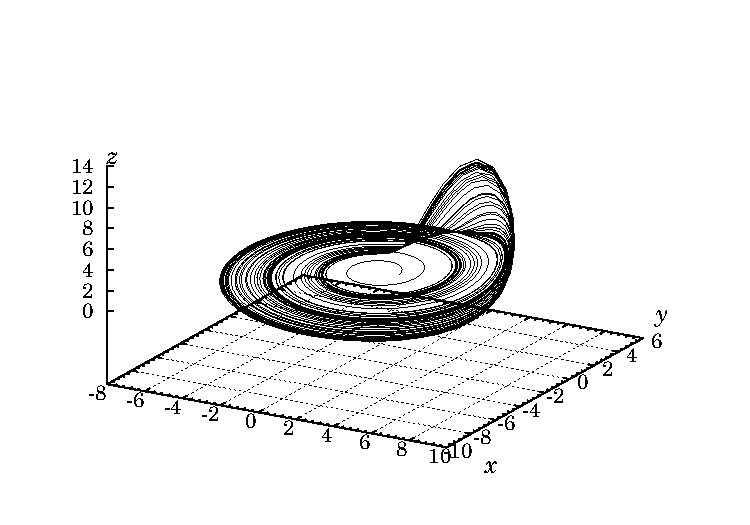
\includegraphics[width=0.6\textwidth]{p/cha/ross_phase3.pdf} }
\caption{Аттрактор системы Рёсслера (\ref{atu:eq:rossler})}
\label{atu:f:ross_phase}
\end{figure}

% }}}2

\subsection{Анализ критериев}  % {{{2

Критерий
$ z_{\max}$, $ \overline{z} $.

% }}}2

\subsection{Тестовая задача идентификации для системы Рёсслера}  % {{{2


% }}}2

\subsection{Влияние параметров системы идентификации на ошибку идентификации для системы Рёсслера}  % {{{2

% }}}2

\subsection{Зависимости значений критериев идентификации при изменении двух параметров системы Рёсслера}  % {{{2

% }}}2



\subsection{Выводы}  % {{{2

Выводы

% }}}2


% }}}1

% vim: fdm=marker ft=tex
 % ??


\FloatBarrier
\subsection{Система Ван-дер-Поля} % _VDP_

\LinkRef{
  vdp: ASAU-16, 17(alt), ITMM-2011
}

\begin{equation}
 \ddot{x} - \varepsilon (1-x^2)  \dot{x} + \Omega_0^2 x  = u(t) .
\label{atu:eq:vdp}
\end{equation}

\( u(t) = U_{in} \sin ( \omega_{in} t ) \),

Идентифицируемый параметр:
\( \varepsilon \in [1;2]  \)

Остальные параметры:
\(U_{in}=0.3\),
\(\omega_{in}=0.2715\).


\begin{figure}[htb!]
\centerline{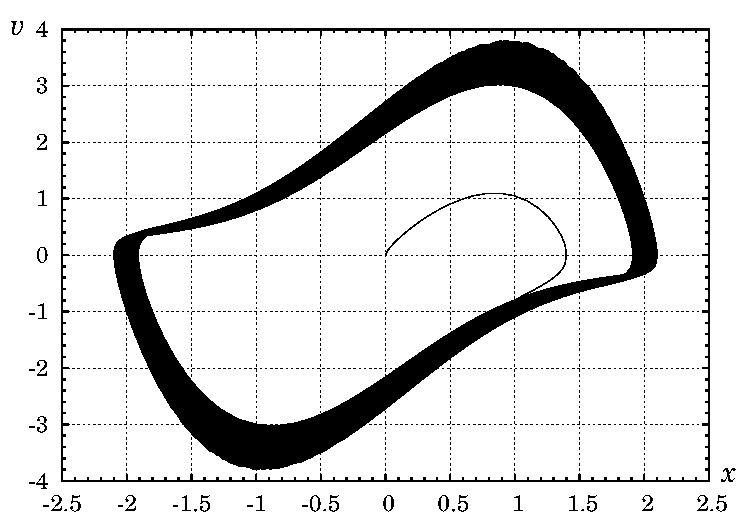
\includegraphics[width=0.5\textwidth]{p/cha/vdp_phase.pdf} }
\caption{Фазовый портрет системы Ван-дер-Поля (\ref{atu:eq:vdp})}
\label{atu:f:vdp_phase}
\end{figure}

Критерий:
$\overline{T}$ + люфт + sign.

Альтернативный критерий:
$\overline{x^2}$


 % ??

\FloatBarrier
\section{Генератор Колпитца} % _COLP_

\LinkRef{
  colp: ASAU-21, APIR-2013
}

В ряде радиоэлектронных устройств используются
генераторы сигналов, способные генерировать разнообразные виды  сигналов, в том числе
сложно-периодические и хаотические.
В частности, генератор  Колпитца~\cite{kennedy_chaos_colpitts,atu_asau21}, который, в
зависимости от условий,   может
генерировать  колебания,  как  близкие  к  гармоническим,  так  и  проявлять
хаотическую  динамику  в  широком  спектральном   диапазоне.   Идентификация
параметров рассматриваемого генератора  необходима,  с  одной  стороны,  для
обеспечения  требуемых  режимов  работы.  С  другой  стороны,  информация  о
параметрах системы необходима при проведении  контроля  работоспособности  в
процессе эксплуатации устройства~\cite{atu_apir2013}.

На рис.~\ref{atu:f:colp_schem} приставлена одна из электрических схем,
реализующих генератор Колпитца на биполярном транзисторе.
Из множества схем, данная была выбрана из-за наличия
одного источника напряжения и простоты схемотехнической реализации генератора.


\begin{figure}[htb!]
\begin{center}
% vi:syntax=tex

\begin{circuitikz}[line width=0.7]
  \ctikzset{bipoles/thickness=2}
  \def\Top{8.0}
  %
  \draw (3.0,3.0) node[npn](npn) {};
  \draw (2.8,3.0) circle[radius=0.5];
  %\draw (npn.center) circle[radius=0.5];
  %
  \draw (0.0,0.0)
   to[R,l=$R_2$,-*]  (0.0,3.0)
   to[R,l=$R_1$]     (0.0,\Top)
   to[short]         (6.0,\Top)
   to[battery,l=$V_{cc}$] (6.0,0.0)
   -- (0.0,0.0);
  %
  \draw (1.5,0.0) to[C,l=$C_0$,*-*] (1.5,3.0);
  \draw (0.0,3.0) -- (npn.base);
  \draw (3.0,0.0) to[vR,l=$R_e$,*-*] (3.0,2.0)
   to[short] (npn.emitter);
  \draw (npn.collector)
   to[L,l=$L$,i<=$I_L$] (3.0,6.0)
   to[R,l=$R_c$] (3.0,\Top);
  %
  \draw (4.5,0.0) to[C,l=$C_2$,v=$V_2$,*-*] (4.5,2.0);
  \draw (4.5,2.0) -- (3.0,2.0);
  \draw (4.5,2.0) to[C,l=$C_1$,v=$V_1$]     (4.5,4.0);
  \draw (4.5,4.0) -- (3.0,4.0);
  \filldraw (3.0,4.0) circle[radius=0.05];
\end{circuitikz}



%\begin{tikzpicture}[circuit ee IEC,very thick,circuit symbol unit=2.5mm]
%%\tikzset{circuit declare symbol=transistor}
%%\tikzset{set transistor graphic=transistor IEC graphic}
%  \node (R2)    at (0.0,0.0) [elelem,point up,resistor={info = $R_2$}] {};
%  \node (pR1R2) at (0.0,1.5) [contact] {};
%  \node (R1)    at (0.0,3.0) [elelem,point up,resistor={info = $R_1$}] {};
%  %
%  \node (C0)    at (1.5,0.0) [point up,elelem,capacitor={info = $C_0$}] {};
%  \node (pR2C0) at (1.5,1.5) [contact] {};
%  %
%  \node (Re)    at (3.0,0.0) [elelem,point up,resistor={adjustable,info = $R_e$}] {};
%  %\node (Q1)    at (3.0,1.5) [elelem,point right,transistor] {};
%  \node (L)     at (3.0,3.0) [elelem,point up,inductor={info = $L$}] {};
%  \node (Rc)    at (3.0,4.5) [elelem,point up,resistor={info = $R_c$}] {};
%  %
%  \node (C2)    at (4.5,0.0) [point up,elelem,capacitor={info = $C_2$}] {};
%  \node (C1)    at (4.5,3.0) [point up,elelem,capacitor={info = $C_1$}] {};
%  %
%  \node (Bat)   at (6.0,0.0) [point up,elelem,battery={info = $Vcc$}] {};
%\end{tikzpicture}


\end{center}
\caption{Электрическая схема генератора Колпитца на биполярном транзисторе}
\label{atu:f:colp_schem}
\end{figure}

При создании модели генератора Колпитца систему уравнений можно
заранее упростить, если заметить, что
делитель на резисторах
$\mathrm{R}_1$, $\mathrm{R}_2$,
вместе с конденсатором
$\mathrm{C}_0$ обеспечивают
постоянство потенциала базы
$V_b = V_{CC} \frac{R_1}{R_1+R_2}$,
поэтому из дальнейшего рассмотрения данные элементы следует
исключить.

Рассмотрев процессы заряда конденсаторов и изменение тока через
катушку индуктивности, получим следующую систему уравнений:
%
\begin{equation}
\label{atu:eq:colp_phys}
\begin{dcases}
  C_1 \od{V_{1}}{t}  = I_L - I_{CE} , \\
  L\, \od{I_L}{t} \; = V_{CC} - V_{1} - V_{2} - I_L R_C , \\
  C_2 \od{V_{2}}{t}  = I_L - \frac{V_{2}}{R_e}.
\end{dcases}
\end{equation}
%
%
%\noindent
где
$V_{CC} $ -- напряжение питания,
$V_1,$ $V_2$ -- разность потенциалов между выводами конденсаторов
$\mathrm{C}_1$ и $\mathrm{C}_2$ соответственно,
$I_L$, $I_{CE}$ -- токи катушки индуктивности и транзистора (коллектор-эмиттер).

Перейдём к безразмерным величинам.
При переходе к безразмерному виду следует определить,
какие физические параметры определяют безразмерные величины.
Это потребуется для синтеза критерия идентификации.
Для упрощения рассмотрения, не снижая общности,
будем считать $C_1 = C_2 = C$.

Прежде всего, воспользуемся тем, что система содержит только один
активный нелинейный компонент -- транзистор.
Следовательно, именно этот элемент определяет
масштаб по напряжению. В простейшей модели транзистора
такой масштабной величиной может служить
$V_{je}$ -- падение напряжения на переходе база-эмиттер
в активном режиме. Следовательно, все разности потенциалов в схеме можно нормировать
на эту величину.

Динамические свойства (в т.ч. условия начала генерации и перехода в хаотический режим) определяются
соотношением активных и реактивных свойств системы. При этом величина
$ \rho = \sqrt{L/C} $ имеет размерность сопротивления
и определяет величину реактивного сопротивления. Эту величину можно использовать
для обезразмеривания активных сопротивлений.

Для приведения токов к безразмерному виду, с учётом уже выбранных величин,
следует использовать величину $ V_{je} / \rho$.


Исходя из всего вышеперечисленного, обозначим:
%
\[
  x = \frac{V_{1}}{V_{je}} ; \quad
  y = \frac{\rho I_L}{V_{je}} ; \quad
  z = \frac{V_{2}}{V_{je}}, \quad
  i_{ce} = \frac{\rho I_{ce}}{V_{je}}, \quad
  c = \frac{V_{CC}}{V_{je}}, \quad
  e = \frac{V_{b}}{V_{je}}.
\]
%
\[
  b = \frac{R_c}{\rho}; \quad
  d = \frac{\rho}{R_e}. % sic!
\]

Система уравнений принимает вид:
%
\begin{equation}
\label{atu:eq:colp_phys2}
\begin{dcases}
  \od{x}{t}  = \dfrac{1}{\rho C}  y - \dfrac{1}{\rho C} i_{ce} , \\
  \od{y}{t}  = \dfrac{\rho}{L} c    - \dfrac{\rho}{L} r_c y - \dfrac{\rho}{L} x- \dfrac{\rho}{L} z, \\
  \od{z}{t}  = \dfrac{1}{\rho C}  y - \dfrac{1}{\rho C} \dfrac{1}{r_e} z.
\end{dcases}
\end{equation}

Общий множитель $ \frac{1}{\rho C} = \frac{\rho}{L} = \sqrt{\frac{1}{LC}} $ в правых частях уравнений
естественным образом задаёт масштаб по времени.
Это подчёркивает, что частотные характеристики рассматриваемого генератора,
в отличие, например, от релаксационного,
определяются ёмкостью и индуктивностью,
поэтому масштаб времени задаём так:
$ T_s = \sqrt{L C} $.
Тогда безразмерное время $t_s$
и соответствующие производные
будут определяться как:
%
\[
  t_s = \frac{t}{T_s}; \quad
  \mathrm{d}\, t = T_s \mathrm{d}\, t_s; \quad
  \od{}{t}  = \frac{1}{T_s} \od{}{t_s}; \quad
  \od{x}{t_s} \equiv \dot{x} = T_s \od{x}{t} .
\]

Поведение величины $I_{ce}$ (в дальнейшем просто $I_c$) достаточно хорошо описывает модель
Эберса-Молла~\cite{horowitz}:
%
\begin{equation}
  I_c = I_s \left( \exp\frac{V_{be}}U_t{} - 1 \right),
  \label{atu:eq:ebers-moll}
\end{equation}
%
%\noindent
где
$I_s$ -- ток насыщения (паспортная или определяемая экспериментально величина),
$U_t=kT/q$,
$q = \SI{1.6e-19}{\coulomb}$ -- заряд электрона,
$k = \SI{1.38e-23}{\joule/\kelvin}$ -- постоянная Больцмана.
Необходимо учесть, что в режиме отсечки ($V_b < V_e$) ток коллектора пренебрежимо мал,
а в режиме насыщения определяется другими элементами схемы.
Существуют и более сложные модели, например,
программы для моделирования электронных схем часто используют так называемую SPICE модель.

К сожалению, при моделировании генератора Колпитца в литературе,
посвящённой хаотической динамике, используют
простейшую модель транзистора, считая, что переход
база-эмиттер открывается при $V_{BE} = V_{je}$, $ I_c \gg I_b$,
а ток коллектора
%
\begin{equation}
I_c =
  \begin{cases}
    \alpha ( V_b - V_e - V_{je} ), & V_b - V_e > V_{je} \\
    0                              & \text{otherwise}.
  \end{cases}
  \label{atu:eq:bjt_libear_model}
\end{equation}



С учётом всего вышеизложенного получаем следующую систему уравнений:
%
\begin{equation}
\label{atu:eq:colp}
\begin{cases}
  \dot{x} = y - a F(z), \\
  \dot{y} = c - x - by - z, \\
  \dot{z} = y - d z.
\end{cases}
\end{equation}

При этом параметр $b$ характеризует соотношение
активного и реактивного сопротивления,
и, следовательно, режима работы генератора.
Величиной этого параметра проще всего управлять,
изменяя $R_c$.
Ставится задача идентификации данного параметра.

При физическом моделировании, проведённом в рамках данной работы использовались следующие
элементы с соответствующими параметрами:
%
\[
  V_{cc} = \SI{12.06}{\volt},          \;
  R_1 = R_2 = \SI{2.2}{\kilo\ohm},     \;
  R_e = \SI{430}{\ohm},
\]
%
\[
  C_1 = C_2 = \SI{1.03}{\micro\farad}, \;
  L = \SI{6.22}{\milli\henry},         \;
  T = \SI{305}{\kelvin},
\]
%
\[
  \text{Q: 2N2222A}, \quad
  h_{fe}=285, \;
  V_f = \SI{0.677}{\volt}, \;
  I_s = \SI{9.61e-14}{\ampere}, \;
  \alpha \approx 1.
\]

Тогда безразмерные коэффициенты:
\[
 a = 77,     \quad
 c = 18.08,  \quad
 d = 0.19,   \quad
 e = 9.07.
\]
%
\[
F(z) =
\begin{cases}{l}
  e-1-z, & z \le e-1  \\
  0,     & z  >  e-1
\end{cases}.
\]


Диапазон изменения идентифицируемого параметра
$b \in [ 0.02; 4.2 ]$
определяется, с одной стороны, собственным сопротивлением катушки индуктивности,
с другой -- срывом генерации.


На рис.~\ref{atu:f:colp_real_xzz}--\ref{atu:f:colp_model_f} предствлены как результаты реального эксперимента,
так и данные, полученные в результате численного моделирования динамики системы (\ref{atu:eq:colp}).
Представлены проекции аттракторов на плоскость $(x+z,z)$ (естественный вид для оциллографа),
трёхмерный вид аттракторов, и спектры.
На каждом рисунке представлено три режима: обычный, момент первого удвоения периода и хаотический режим.


\begin{figure}[htb!]
 \centerline{
   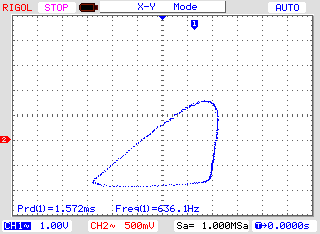
\includegraphics[width=0.32\textwidth]{p/cha/colp/colp_m1_vv.png}
   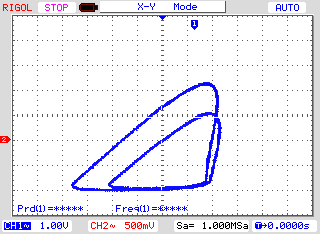
\includegraphics[width=0.32\textwidth]{p/cha/colp/colp_m2_vv.png}
   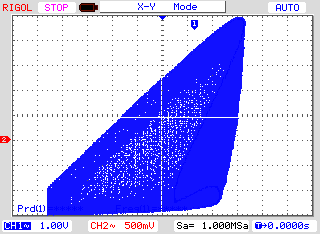
\includegraphics[width=0.32\textwidth]{p/cha/colp/colp_m3_vv_ac.png}
 }
  \caption{Проекции аттракторов реальной системы Колпитца на плоскость $(x+z,z)$
  для трёх режимов}
  \label{atu:f:colp_real_xzz}
\end{figure}

\begin{figure}[htb!]
 \centerline{
   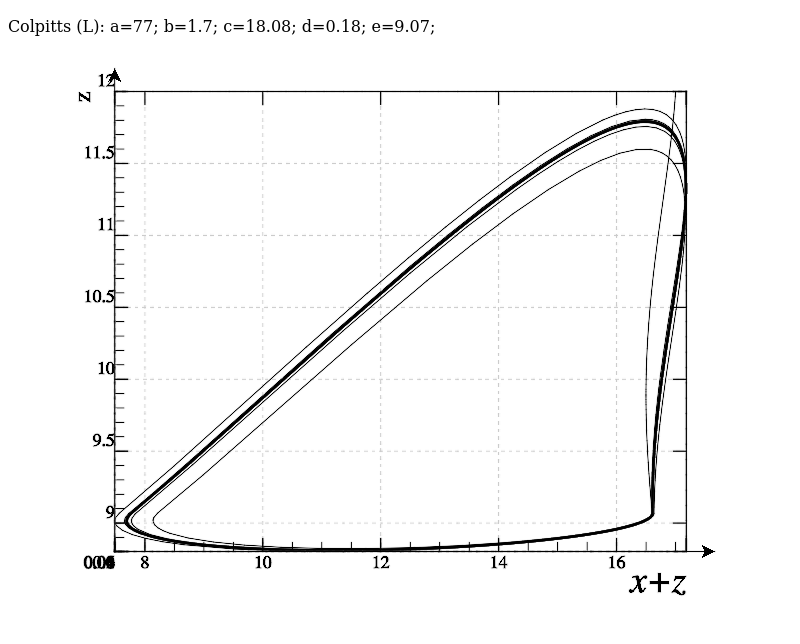
\includegraphics[width=0.32\textwidth]{p/cha/colp/colp_0-p_z_xpz_b=1x70.png}
   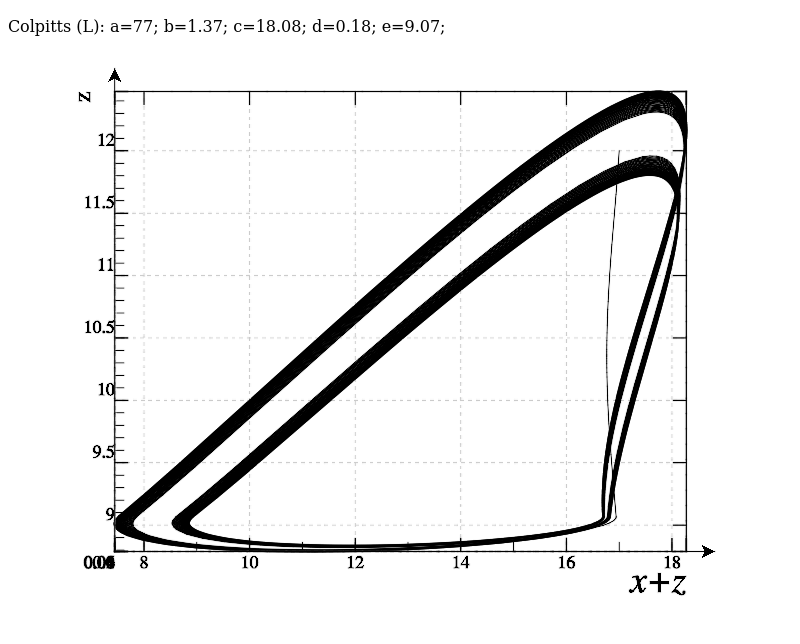
\includegraphics[width=0.32\textwidth]{p/cha/colp/colp_0-p_z_xpz_b=1x37.png}
   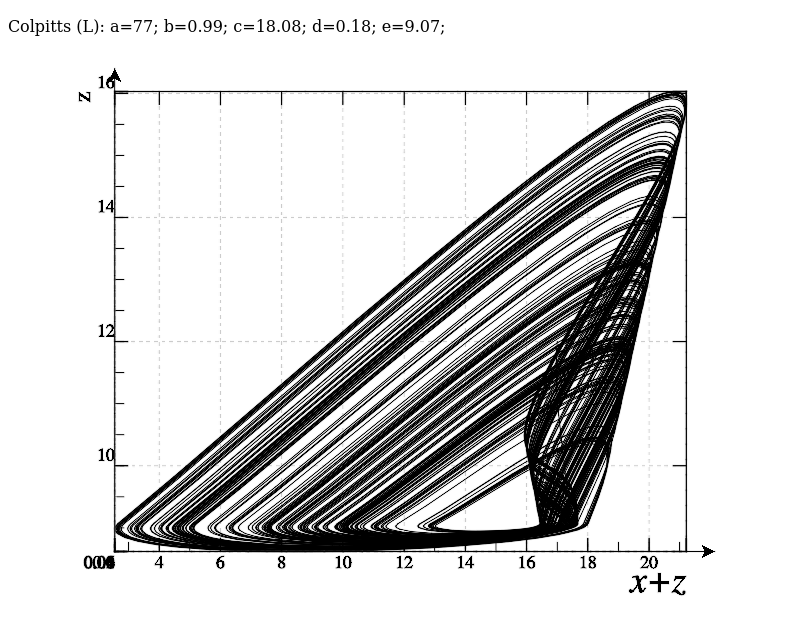
\includegraphics[width=0.32\textwidth]{p/cha/colp/colp_0-p_z_xpz_b=0x99.png}
 }
  \caption{Проекции аттракторов модели (\ref{atu:eq:colp}) системы Колпитца на плоскость $(x+z,z)$
  для трёх режимов}
  \label{atu:f:colp_model_xzz}
\end{figure}


\begin{figure}[htb!]
 \centerline{
   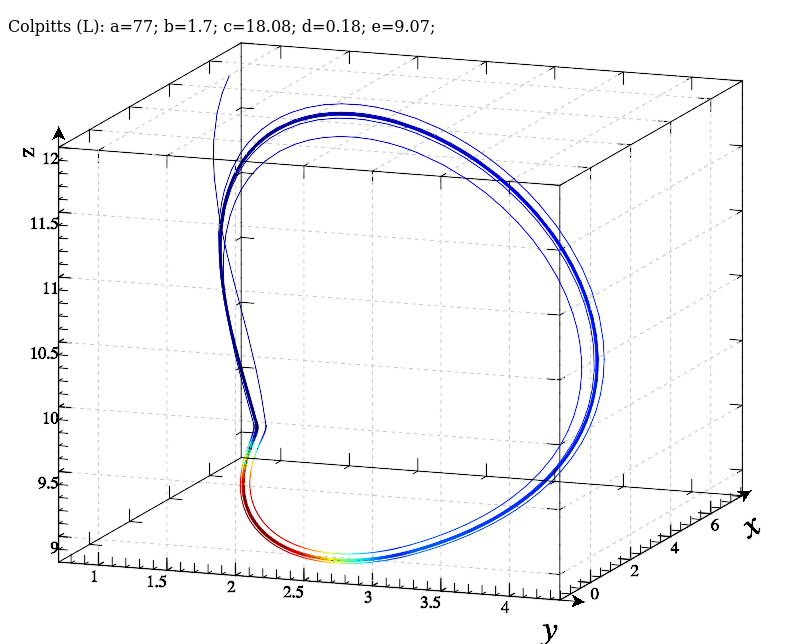
\includegraphics[width=0.32\textwidth]{p/cha/colp/colp_0-p_xyz_b=1x70.png}
   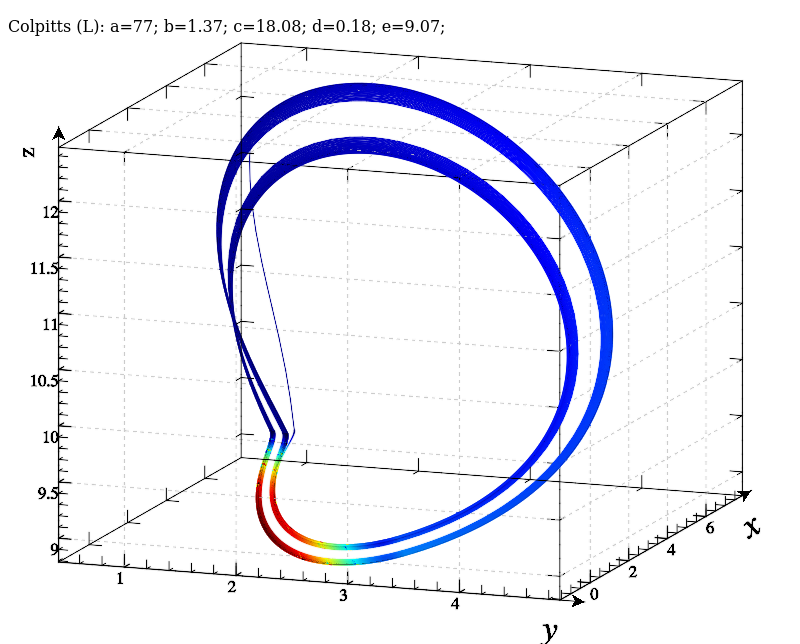
\includegraphics[width=0.32\textwidth]{p/cha/colp/colp_0-p_xyz_b=1x37.png}
   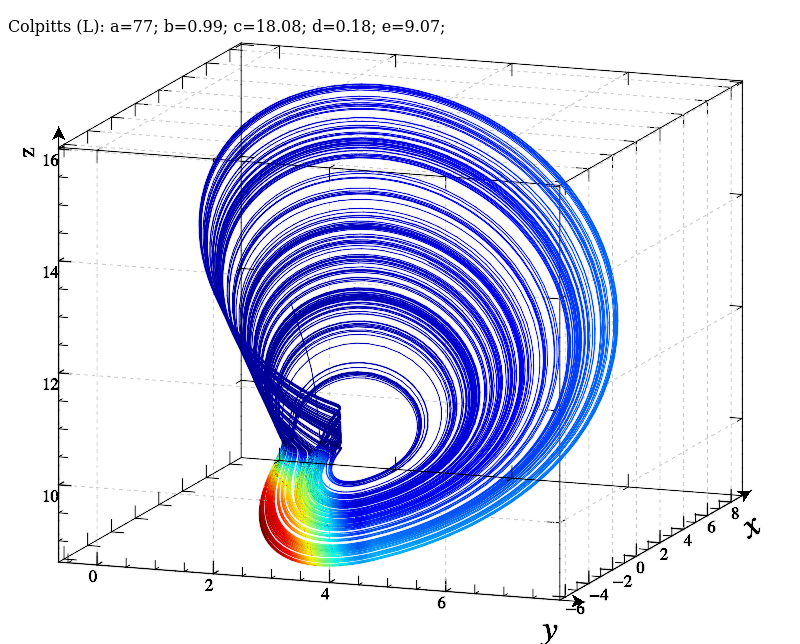
\includegraphics[width=0.32\textwidth]{p/cha/colp/colp_0-p_xyz_b=0x99.png}
 }
  \caption{Аттрактороы модели (\ref{atu:eq:colp}) системы Колпитца для трёх режимов}
  \label{atu:f:colp_model_xyz}
\end{figure}

\begin{figure}[htb!]
 \centerline{
   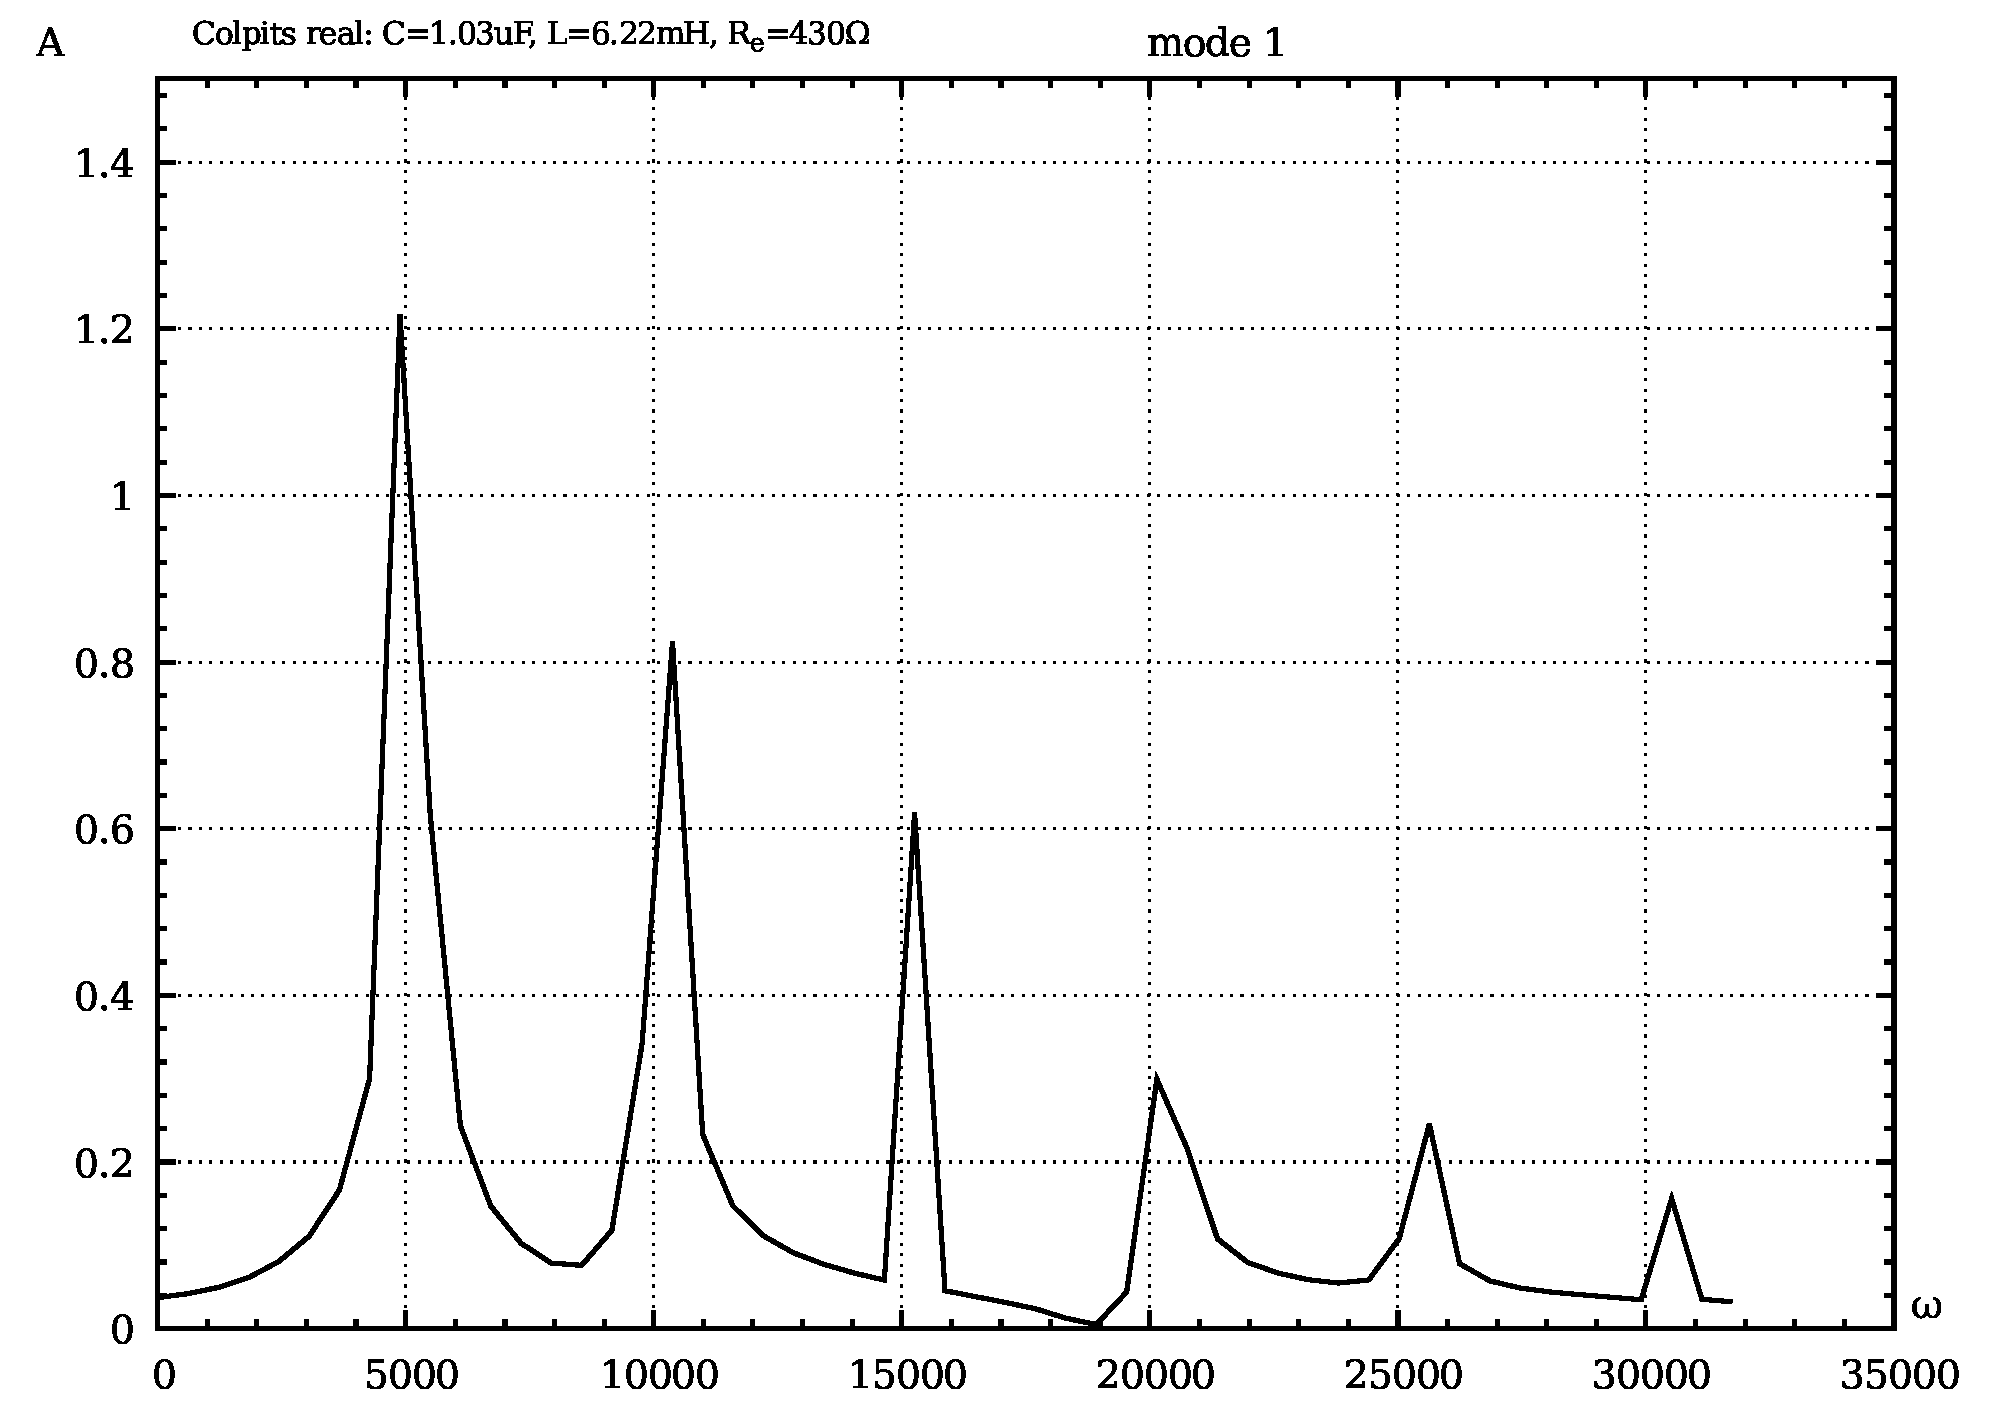
\includegraphics[width=0.32\textwidth]{p/cha/colp/colp_m1_f.png}
   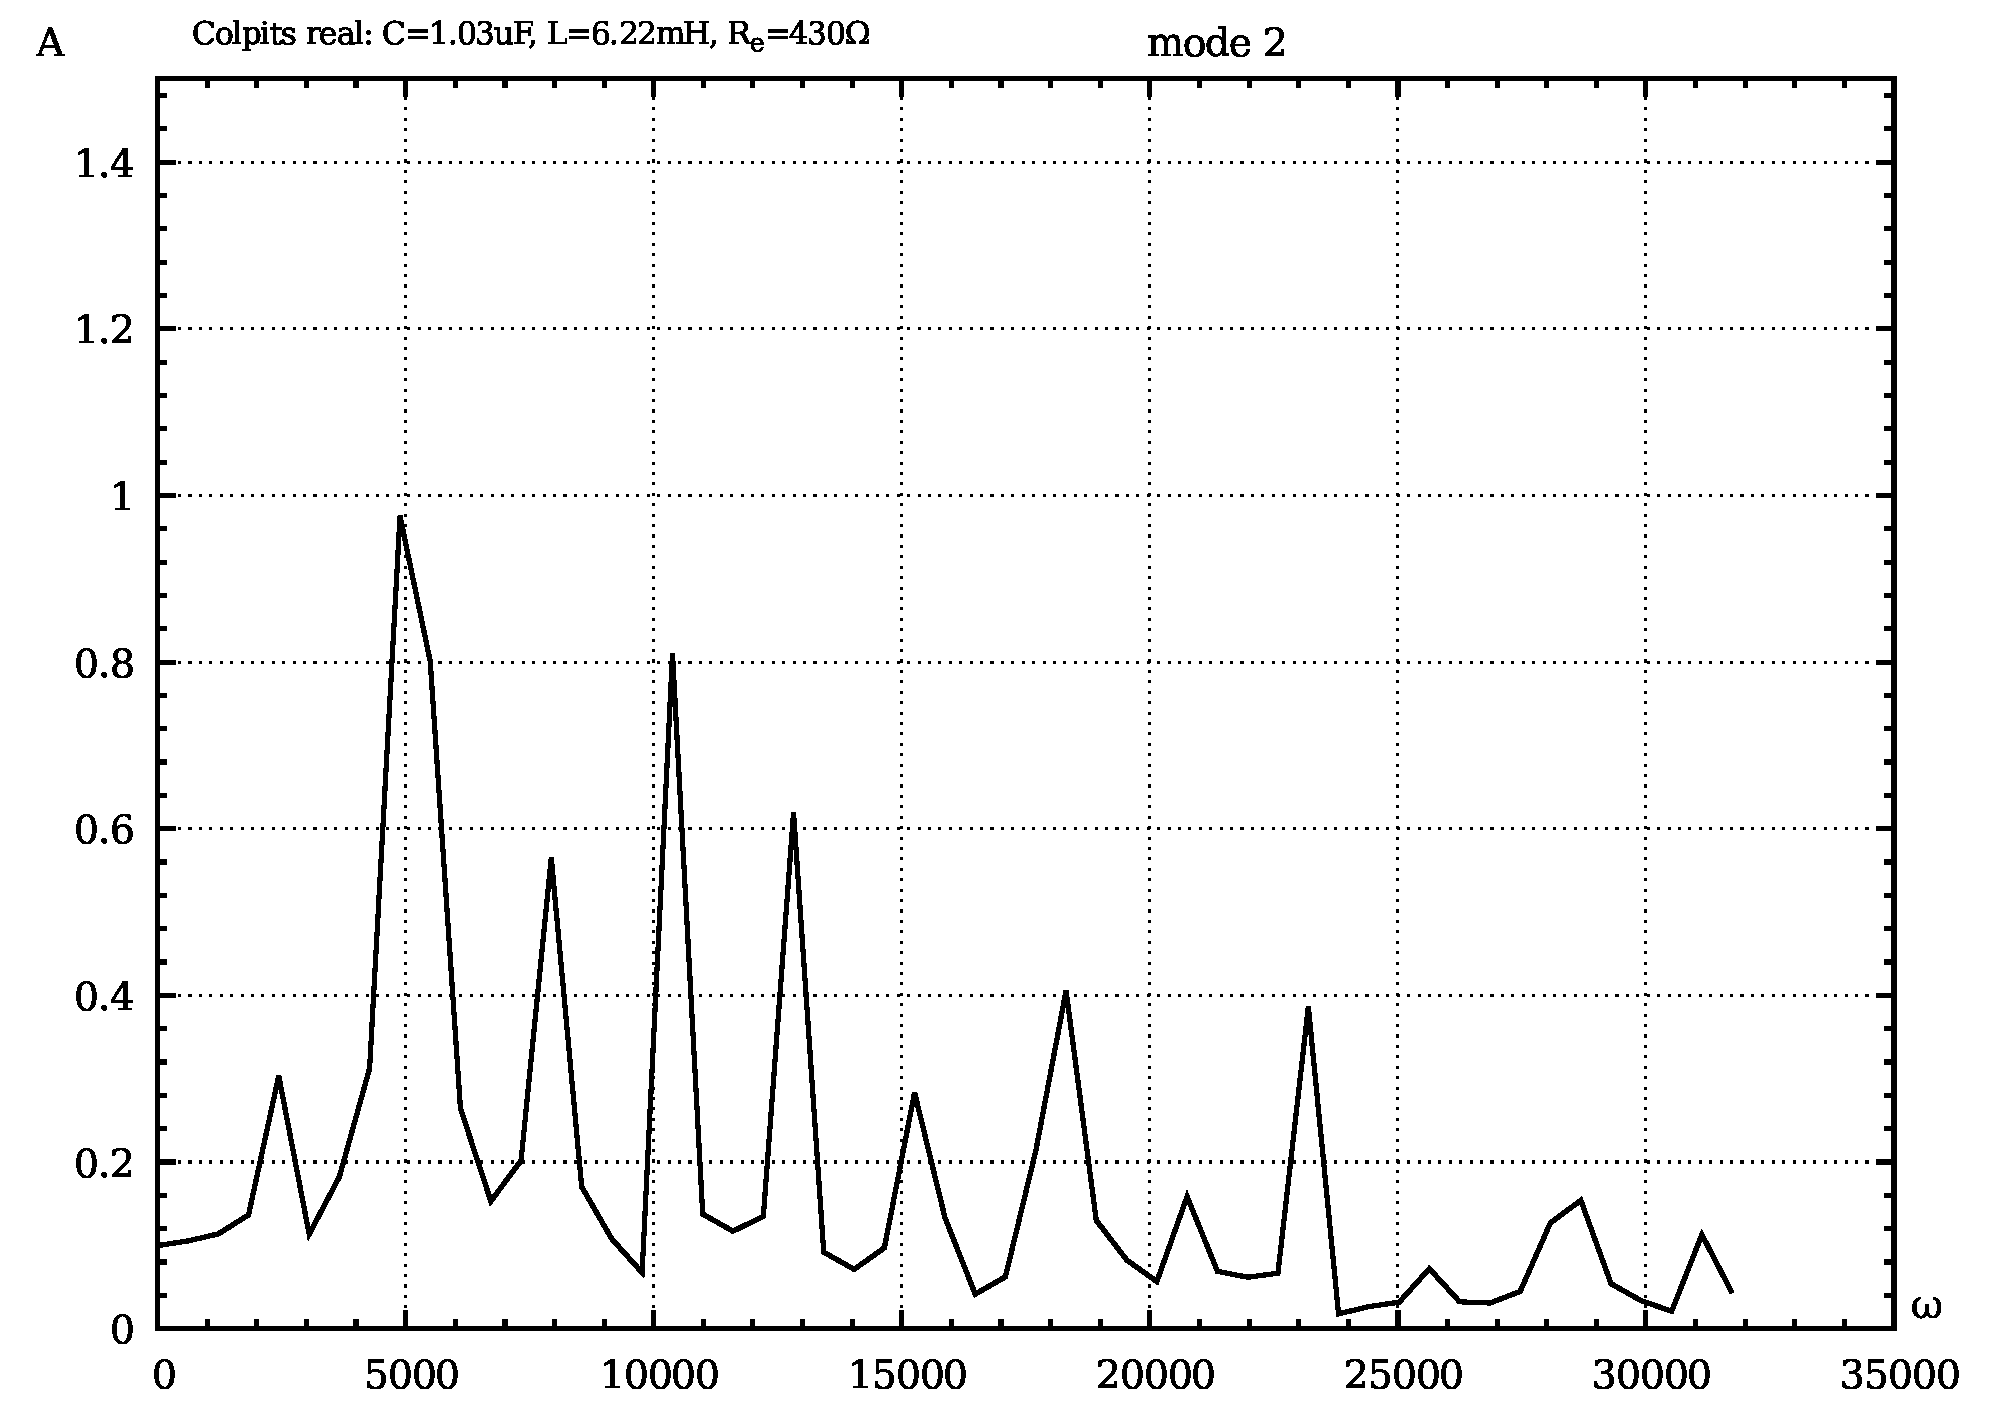
\includegraphics[width=0.32\textwidth]{p/cha/colp/colp_m2_f.png}
   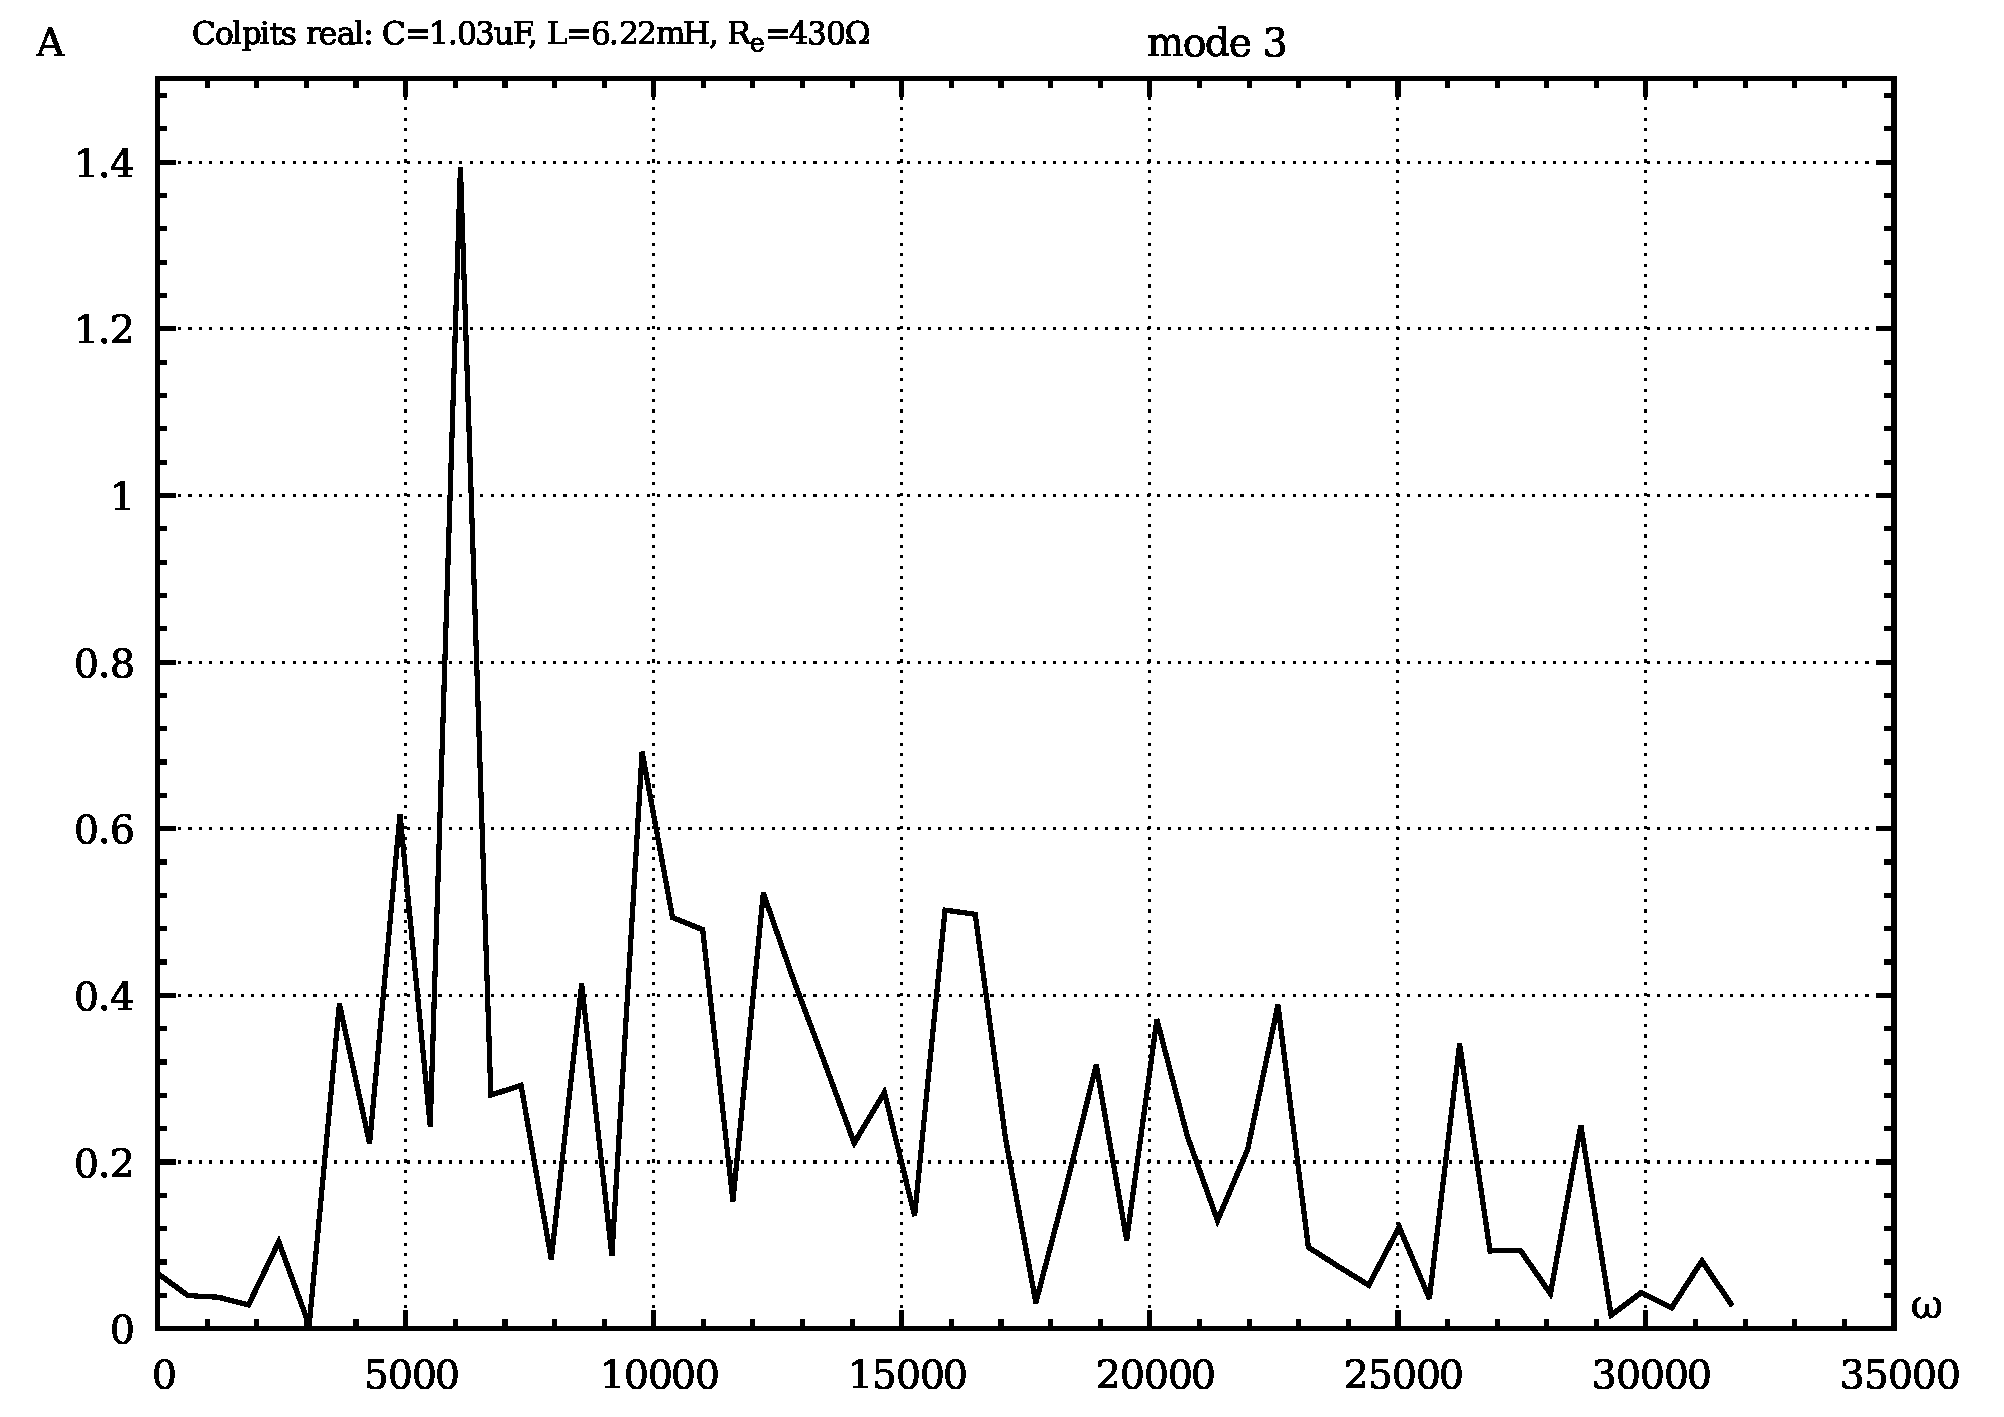
\includegraphics[width=0.32\textwidth]{p/cha/colp/colp_m3_f.png}
 }
  \caption{Спектры реальной системы Колпитца  для трёх режимов}
  \label{atu:f:colp_real_f}
\end{figure}

\begin{figure}[htb!]
 \centerline{
   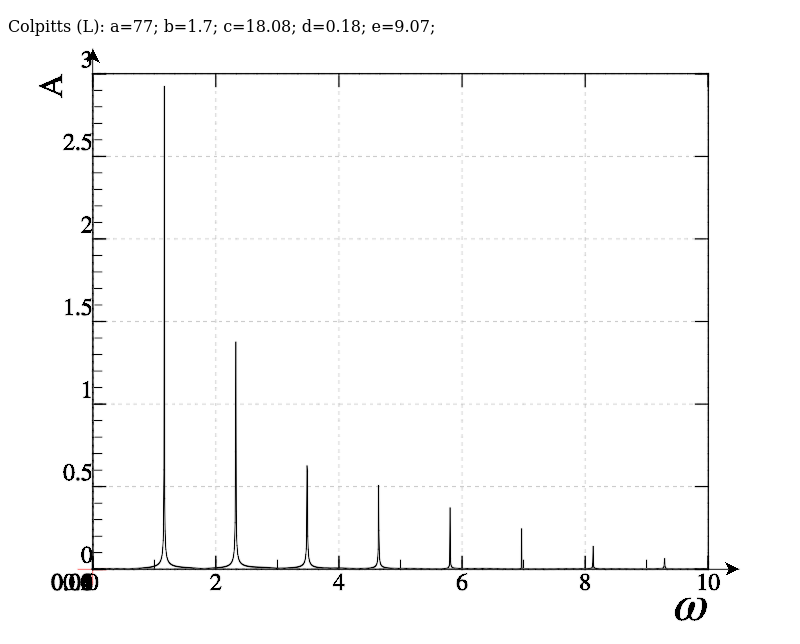
\includegraphics[width=0.32\textwidth]{p/cha/colp/colp_f-p_f_b=1x70.png}
   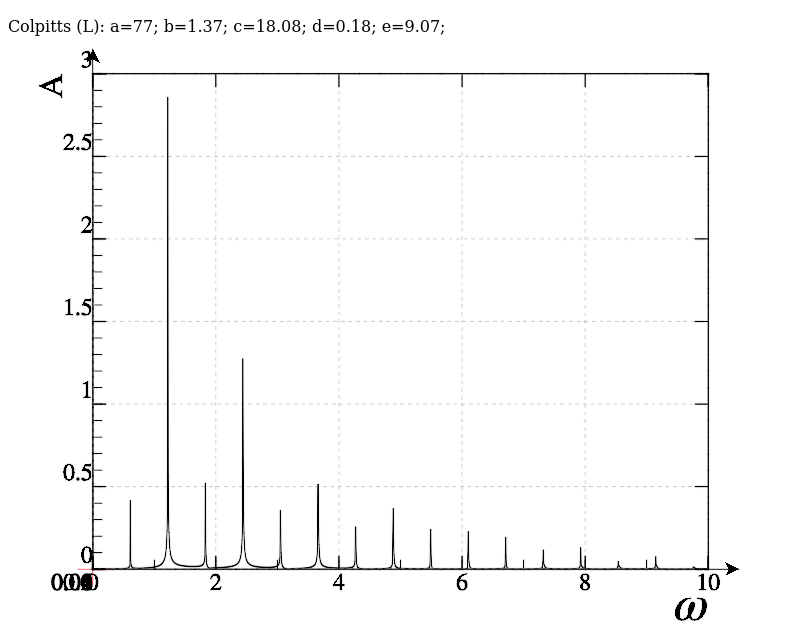
\includegraphics[width=0.32\textwidth]{p/cha/colp/colp_f-p_f_b=1x37.png}
   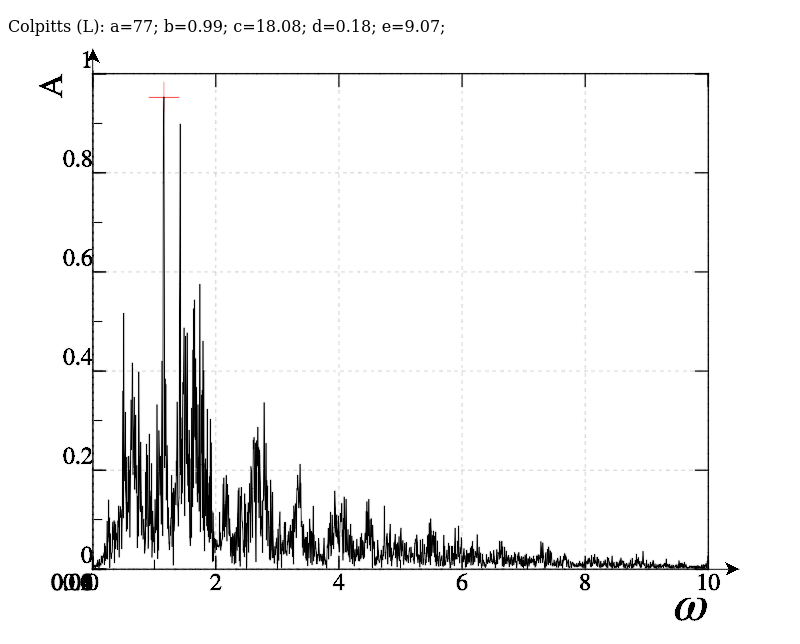
\includegraphics[width=0.32\textwidth]{p/cha/colp/colp_f-p_f_b=0x99.png}
 }
  \caption{Спектры модели (\ref{atu:eq:colp}) системы Колпитца для трёх режимов}
  \label{atu:f:colp_model_f}
\end{figure}

Сравнение результатов физического и численного моделирования позволяет сделать вывод
о качественном подобии поведения реальной системы и модели.
Тем не менее, величины параметра $b$, при которых получены
рассматриваемые режимы, совпадают весьма приближённо.
Для реальной системы значения параметра: $b = 1.06, \; 0.94, \; 0.90 $, в то время как
для модели: $b = 1.70, \; 1.34, \; 0.99 $.
Расхождение значений, скорее всего, связано с грубостью модельного представления (\ref{atu:eq:bjt_libear_model}) транзистора.
Вопрос применимости различных моделей биполярного транзистра в рамках рассмативаемой системы
требует дальнейшего исследования.
С другой стороны, ограниченный набор данных, получаемых с осциллографа Rigol DS1052E (8192 отсчёта) не позволяют
получить достаточно подробный спектр реальной системы.

Для определения критерия идентификации рассмотрим зависимости
$q_{*}(\mu) $, полученные путём моделирования
для системы Колпитца (рис.~\ref{atu:f:colp_q}).
При этом следует учесть, что наиболее просто измеряемыми величинами являются $x$ и $z$,
соответствующие напряжениям $V_1$ и $V_2$.
Первый набор зависимостей даёт два основных кандидата -- $q_{x^2}$ и $q_{z^2}$.
При этом первый из них показывает более равномерную зависимость.
В то же время, большинство из рассморенных зависимостей имею явно
выраженный гиперболический характер, особенно при малых значениях $b$.
Следовательно, в список кандидатов следует добавить $q_{x^{-2}} $ и $q_{z^{-2}}$.

\begin{figure}[htb!]
\centerline{
  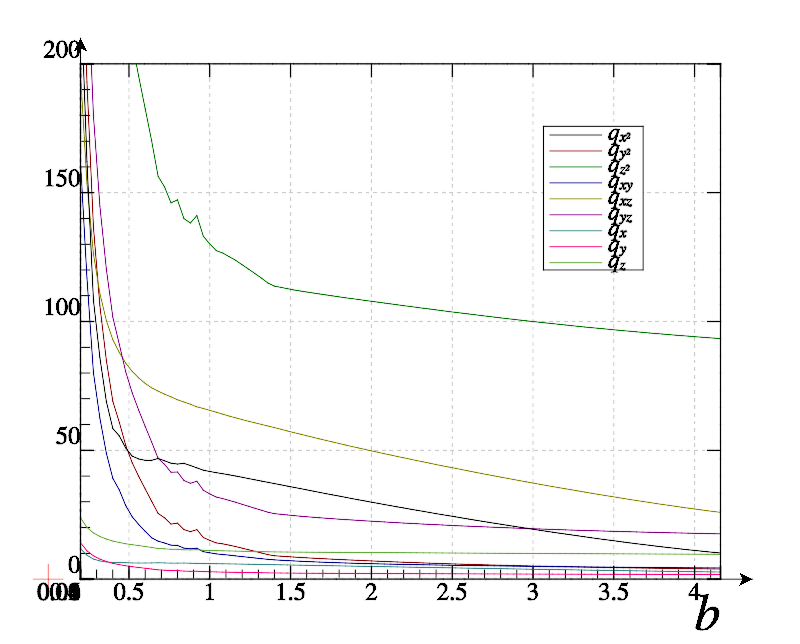
\includegraphics[width=0.49\textwidth]{p/cha/colp/colp_p-p_b_e.png}
  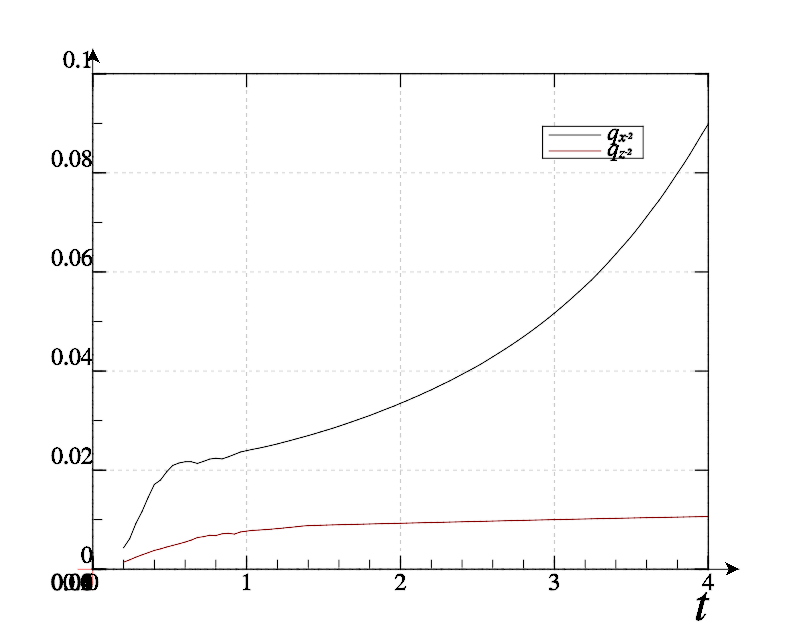
\includegraphics[width=0.49\textwidth]{p/cha/colp/colp_p-p_b_1ex2.png}
}
  \caption{Зависимости $q_{*}(b) $ для системы Колпитца (\ref{atu:eq:colp})}
\label{atu:f:colp_q}
\end{figure}

Из графиков очевидно, что
обратные зависимости не дают заметного выигрыша, поэтому выберем
величину $ q_{x^2}(b) $ в качестве критерия.

В качестве системы идентификации использовалась система с пятью поисковыми агентами и
двумя неподвижными моделями. Аналогично предыдущим системам,
для исследования динамических свойств системы идентификации
изменения параметра $b_o$ как:
%
\begin{equation}
 b_o(t) = p_0 + U_p \sign \sin( \omega_p t ),
  \label{atu:eq:colp_b_sign}
\end{equation}
%
\begin{equation}
 b_o(t) = p_0 + U_p \sin( \omega_p t ).
  \label{atu:eq:colp_b_sin}
\end{equation}

Динамика процессов идентификации для системы Колпитца представлена на рис.~\ref{atu:f:colp_id}.

\begin{figure}[htb!]
\centerline{
  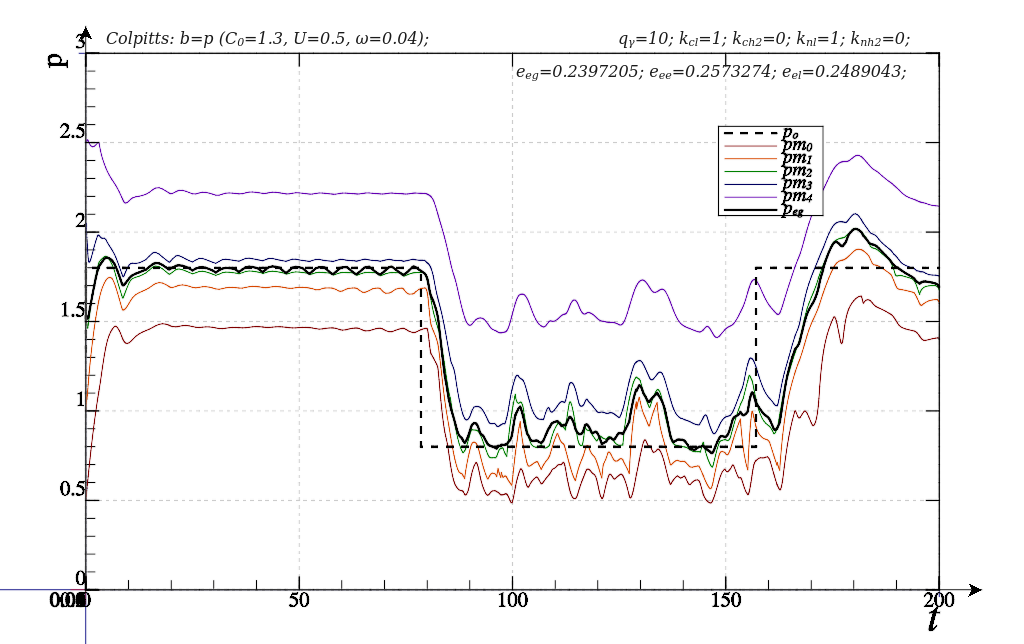
\includegraphics[width=0.49\textwidth]{p/cha/colp/colp_m5p-pl_n_sign.png}
  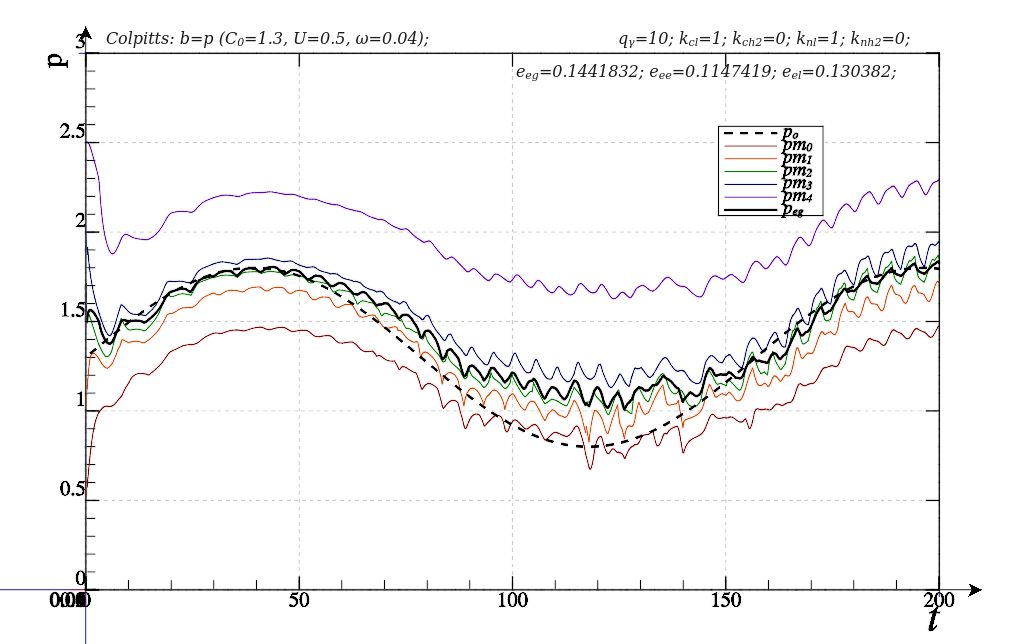
\includegraphics[width=0.49\textwidth]{p/cha/colp/colp_m5p-pl_n_sin.png}
}
\caption{Процесс идентификации параметра $b$ системы (\ref{atu:eq:colp})
  при условиях (\ref{atu:eq:colp_b_sign}) и (\ref{atu:eq:colp_b_sin})
}
\label{atu:f:colp_id}
\end{figure}

Зависимость среднеквадратических ошибок идентификации от величины $q_\gamma$ (рис.~\ref{atu:f:colp_e_qgamma})
даёт информацию о корректной настройке этого параметра системы идентификации.

\begin{figure}[htb!]
\centerline{
  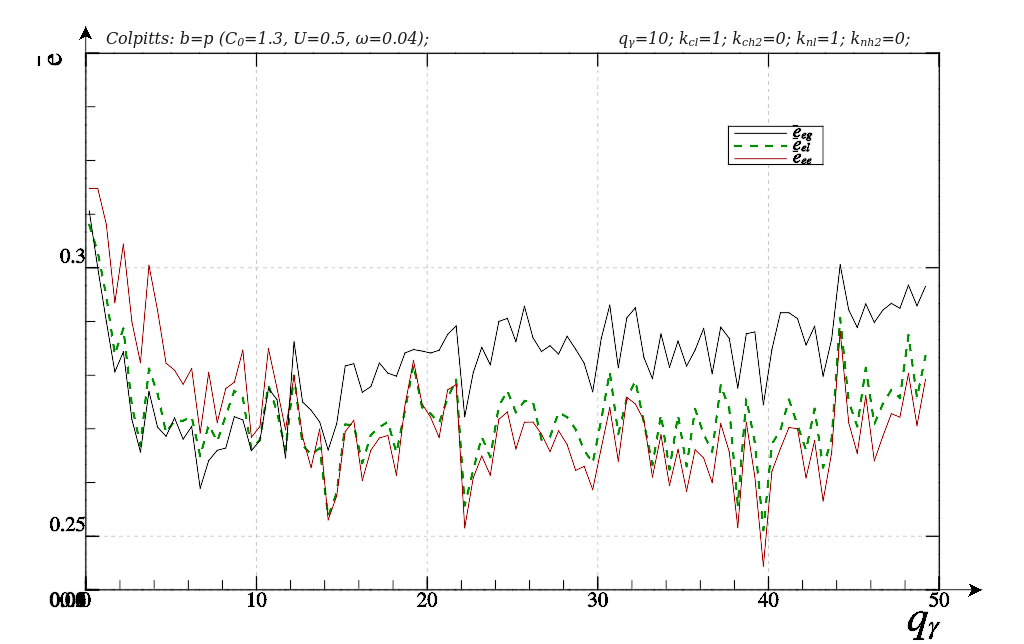
\includegraphics[width=0.49\textwidth]{p/cha/colp/colp_m5p-p_qg_e_sign.png}
  \includegraphics[width=0.49\textwidth]{p/cha/colp/colp_m5p-p_qg_e_sin.png}
}
  \caption{Зависимости  $\overline{e}(q_\gamma)$ для системы (\ref{atu:eq:colp})
  при условиях (\ref{atu:eq:colp_b_sign}) и (\ref{atu:eq:colp_b_sin})
}
\label{atu:f:colp_e_qgamma}
\end{figure}



Аналогично, зависимости $\overline{e_*}(a_q)$ (рис.~\ref{atu:f:colp_e_a_q})
позволяют корректно определить время усреденения.
При этом следует отметить, что
полученные результаты хорошо согласуются со спектрами системы.

\begin{figure}[htb!]
\centerline{
  \includegraphics[width=0.49\textwidth]{p/cha/colp/colp_m5p-p_a_q_e_sign.png}
  \includegraphics[width=0.49\textwidth]{p/cha/colp/colp_m5p-p_a_q_e_sin.png}
}
  \caption{Зависимости  $\overline{e}(a_q)$ для системы (\ref{atu:eq:colp})
  при условиях (\ref{atu:eq:colp_b_sign}) и (\ref{atu:eq:colp_b_sin})
}
\label{atu:f:colp_e_a_q}
\end{figure}

В целом синтез критерия идентификации и построение работоспособной системы идентификации для
системы генератора Колпитца не потребовало никаких специальных подходов и введения дополнительных
мер оценивания взаимосвязей параметров генератора.

 % good


\FloatBarrier

\section{Колебательная с зоной нечувствительности в возвращающей силе} %  % {{{1 _DEADVI_
\label{atu:sect:deadvi}


\subsection{Определение системы и анализ её динамики} %  % {{{2 _deadvi_task

\LinkRef{
  deadvi: ASAU-20, ISDMCI-2013
}

\begin{equation}
\ddot{x} + c_0 \dot{x} + a \cdot x + b \cdot \mathrm{db}(x,x_0) = u(t),
\label{atu:eq:deadvi}
\end{equation}

$ u(t) = U_0 \sin( \omega_{in} t ) $.

Идентифицируемый параметр:
$ x_0 \in [2;2.5] $ -- ширина зоны нечувствительности.

Остальные параметры:
$U_0 = 1.4$, $\omega_{in} = 1.4$, $c_0=0.1$, $a=-0.3$, $b=1.0$.


\begin{figure}[htb!]
\centerline{\includegraphics[width=0.5\textwidth]{p/cha/deadvi_phase.pdf} }
\caption{Фазовый портрет системы ``deadvi'' (\ref{atu:eq:deadvi})}
\label{atu:f:deadvi_phase}
\end{figure}

% }}}2

\subsection{Анализ критериев}  % {{{2

Критерий
$\overline{x^2(t)}$

% }}}2

\subsection{Выводы}  % {{{2

Выводы

% }}}2



% }}}1


% vim: fdm=marker foldlevelstart=3 fdc=4 ft=tex
 %


\FloatBarrier
\subsubsection{Система Sprott A}

\LinkRef{
  spr\_a: MKMM-2016
}

В своих работах J.C.~Sprott рассмотрел целое семейство динамических
систем, реализующих хаотическое поведение, обозначив их латинскими буквами
от ``A'' до ``S''~\cite{sprott_212}. Особое место среди них
занимает система, обозначаемая как ``Sprott A''. Отличительной особенностью
этой системы является отсутствие положений равновесия, что делает
невозможным применение многих известных методов анализа, основанных на
каком-либо разложении в окрестностях точек равновесия. Соответствующая ей
система уравнений имеет вид:

\begin{equation}
  \begin{cases}
    \dot{x} =  y, \\
    \dot{y} = -x + yz, \\
    \dot{z} =  1 - y^2.
  \end{cases}
  \label{atu:eq:spr_a_orig}
\end{equation}


В исходном виде система (\ref{atu:eq:spr_a_orig}) имеет фиксированные значения параметров.
Не изменяя структуры системы, можно ввести 5 параметров, влияющие на её динамку.
Поскольку целью данной работы является определение критериев идентификации параметров
хаотических объектов, для данной системы
работе рассмотрим только один параметр -- $c_{x_y} $. Система принимает следующий вид:

\begin{equation}
  \begin{cases}
    \dot{x} =  c_{x_y} y, \\
    \dot{y} = -x + yz, \\
    \dot{z} =  1 - y^2.
  \end{cases}
  \label{atu:eq:spr_a}
\end{equation}

В таком виде система, при изменении $c_{x_y} $
в достаточно широком диапазоне может демонстрировать как
сложно-периодическое, так и преимущественно, хаотическое
поведение (рис.~\ref{atu:f:spr_a_phase}). При этом, в диапазоне $c_{x_y} \in [0.1 ; 0.7] $
наблюдаются перестройки структуры аттрактора, а при относительно больших
значениях данного параметра аттрактор представляет собой полый тор.


\begin{figure}[htb!]
\centerline{
  \includegraphics[width=0.33\textwidth]{p/cha/spr_a/sprott_a-p_xyz_cx_y=0x372.png}
  \includegraphics[width=0.33\textwidth]{p/cha/spr_a/sprott_a-p_xyz_cx_y=0x610.png}
  \includegraphics[width=0.33\textwidth]{p/cha/spr_a/sprott_a-p_xyz_cx_y=1x000.png}
}
\caption{Аттракторы системы (\ref{atu:eq:spr_a})
  при $ c_{x_y} =0.372 $, $ c_{x_y} =0.61 $, $ c_{x_y} =1.00 $
}
\label{atu:f:spr_a_phase}
\end{figure}

Важной особенностью поведения этой системы является то, что при $ c_{x_y} \ge 1 $
в спектре системы имеются очень ограниченные участки сплошного спектра~(рис.~\ref{atu:f:spr_a_f}).
При этом, как и для получения корректного спектра, так и для обнаружения ``разбегания'' траекторий
необходимо моделирование системы на протяжении достаточно длительного
(по сравнению с многими схожими системами) модельного времени.

\begin{figure}[htb!]
\centerline{
  \includegraphics[width=0.33\textwidth]{p/cha/spr_a/sprott_a_f-p_f_cx_y=0x372.png}
  \includegraphics[width=0.33\textwidth]{p/cha/spr_a/sprott_a_f-p_f_cx_y=0x610.png}
  \includegraphics[width=0.33\textwidth]{p/cha/spr_a/sprott_a_f-p_f_cx_y=1x000.png}
}
\caption{Спектры системы (\ref{atu:eq:spr_a})
  при $ c_{x_y} =0.372 $, $ c_{x_y} =0.61 $, $ c_{x_y} =1.00 $
}
\label{atu:f:spr_a_f}
\end{figure}

Рассмотрим зависимости $q_{*}(c_{x_y}) $ (рис.~\ref{atu:f:spr_a_q})
для системы (\ref{atu:eq:spr_a}). Анализ этих зависимостей
даёт однозначный ответ о возможном виде критерия -- $q_{x^2}$.
Используя его, строим систему идентификации.

\begin{figure}[htb!]
\centerline{
  \includegraphics[width=0.50\textwidth]{p/cha/spr_a/sprott_a_p-p_c_x_y.png}
}
\caption{Зависимости $q_{*}(c_{x_y})$ для системы (\ref{atu:eq:spr_a}) }
\label{atu:f:spr_a_q}
\end{figure}


Динамика процессов идентификации для системы Sprott A представлена на рис.~\ref{atu:f:spr_a_id}.
Общий вид динамики поиска свидетельствует о работоспособности системы.

\begin{figure}[htb!]
\centerline{
  \includegraphics[width=0.49\textwidth]{p/cha/spr_a/sprott_a_m5p-pl_n_sign.png}
  \includegraphics[width=0.49\textwidth]{p/cha/spr_a/sprott_a_m5p-pl_n_sin.png}
}
\caption{Процесс идентификации параметра $c_{x_y} $ системы (\ref{atu:eq:spr_a})
  при различных видах нестационарности этого параметра
}
\label{atu:f:spr_a_id}
\end{figure}

Зависимость среднеквадратических ошибок идентификации от величины $q_\gamma$ (рис.~\ref{atu:f:spr_a_e_qgamma})
свидетельствует о довольно слабом влиянии этого параметра
на динамику системы идентификации.
Проявляются робастные свойства поисковых агентов.

\begin{figure}[htb!]
\centerline{
  \includegraphics[width=0.49\textwidth]{p/cha/spr_a/sprott_a_m5p-p_qg_e_sign.png}
  \includegraphics[width=0.49\textwidth]{p/cha/spr_a/sprott_a_m5p-p_qg_e_sin.png}
}
  \caption{Зависимости  $\bar{e}(q_\gamma)$ для системы (\ref{atu:eq:spr_a})
  при различных видах нестационарности этого параметра
}
\label{atu:f:spr_a_e_qgamma}
\end{figure}


Зависимости $\bar{e_*}(a_q)$ (рис.~\ref{atu:f:spr_a_e_a_q})
с одной стороны, позволяют корректно определить время усреденения,
с другой -- подтверждают тезис о том, что более ярко выраженное изменение
параметра требует большего времени наблюдения за системой
для проведения идентификации.

\begin{figure}[htb!]
\centerline{
  \includegraphics[width=0.49\textwidth]{p/cha/spr_a/sprott_a_m5p-p_a_q_e_sign.png}
  \includegraphics[width=0.49\textwidth]{p/cha/spr_a/sprott_a_m5p-p_a_q_e_sin.png}
}
  \caption{Зависимости  $\bar{e}(a_q)$ для системы (\ref{atu:eq:spr_a})
  при различных видах нестационарности этого параметра
}
\label{atu:f:spr_a_e_a_q}
\end{figure}

Таким образом, для хаотической системы ``Sprott A''
удалось создать и критерий идентификации и работоспособную систему идентификации
на основании энергетического критерия вида (\ref{atu:eq:q}).


 % good


\FloatBarrier
\subsubsection{Система с сухим трением} % __FRIC__

\LinkRef{
  fric: ASAU-11, DSMP-2016
}

Существуют динамические системы, не обладающие хаотическим поведением,
которые, тем не менее, проявляют сходные свойства с точки зрения идентификации.
А именно, непосредственное сравнение выходов системы и модели не позволяет
сделать никаких выводов о соотношениях между параметрами модели и объекта.
Одним из примеров таких систем является динамическая система (\ref{atu:eq:dryfric_sys}),
моделирующая поведение тела заданной массы по действием внешней вынуждающей силы
и силы сухого трения
\cite{berger_friction,atu_asau11}:
%
\begin{equation}
  m \ddot{x} + f_{df}( x, \dot{x}, \ldots)  = u(t).
\label{atu:eq:dryfric_sys}
\end{equation}
%
%\noindent
где
$m$ -- масса тела,
$u(t)$ -- вынуждающая сила,
$ f_{df}( x, \dot{x}, \ldots)  $ -- сила сухого трения.

Важной особенностью при моделировании силы сухого трения является тот факт,
что это силу невозможно корректно выразить аналитически. Более того,
её алгоритмическое представления неизбежно потребует учёта всех других сил,
действующих на тело, то крайней мере, для корректного представления
силы трения покоя. Эта особенность не даёт возможности
аналитического анализа таких систем, за исключением ограниченного набора
вырожденных случаев. При этом, такое поведение существенно затрудняет идентификацию,
и, в определённых случая,х делает её принципиально невозможной.

Основным параметром, в простейшем случае определяющим силу сухого
трения, является $f_{dm}$ -- максимальная значение её модуля.
Определение этой величины и будем считать целью задачи идентификации
системы с сухим трением.

В свою очередь, существенным свойством данной системы является то, что в каждой точке \(x\)
система может находится в покое, даже если на неё действует
внешняя сила (по модулю не превышающая $f_{dm}$).
Если же рассмотреть пару или более подобных систем,
то получившаяся система имеет общие свойства с системами
хаотической динамики, а именно: малые возмущения входного сигнала
или коэффициентов модели приводят к значительным изменениям
выходного, причем реакция на возмущения может быть
не ограничена во времени.
Более того, даже если после какого-то момента времени
параметры объекта и коэффициенты модели полностью совпадут,
величина ошибки по выходнам не устремится к нулю, а останется на прежнем уровне.

На рис.~\ref{atu:f:fric_outs} представлен сравнительный пример динамики трёх
моделей, при одинаковом входном сигнале
и различных значениях $f_{dm}$.

\begin{figure}[htb!]
  \centerline{
    \includegraphics[width=0.5\textwidth]{p/cha/fric/fric_outs.png}
  }
  \caption{Динамика трёх моделей вида (\ref{atu:eq:dryfric_sys})}
  \label{atu:f:fric_outs}
\end{figure}

При дальнейшем моделировании, в качестве сигнала $u(t)$ использовался кусочно-линейный периодический сигнал,
в котором чередуются ``плато'' и резкие изменения. Выбор такой формы обусловлен
характерными режимами работы систем позиционирования электромеханических
устройств, для которых и характерно влияние сухого трения.

Для обеспечения возможности применения методов идентификации,
необходимо существование критерия
\( q(x(t)) \),
удовлетворяющего следующим требованиям:

\begin{itemize}

\item
чувствительность к \textit{динамике} модели и объекта;

\item
свойство астатизма, то есть
независимость
от смещения выхода объекта или модели:
\( q(x(t)+a ) \approx q( x(t) ) \);

\item
достаточная устойчивость к шумам измерения;

\item
физическая реализуемость.

\end{itemize}

Первые два требования
могут быть достигнуты путём вычисления производной --
скорости изменения выходных сигналов
\(v = \mathrm{d}\,x(t)/ \mathrm{d}\,t \),
и формирования критерия идентификации на её основе.

Однако, при этом система становится исключительно чувствительной
к шумам измерения. Даже в том случае, когда
оценка производной производится физически реализуемыми методами,
создать работоспособную систему идентификации на основе критериев
подобного вида практически невозможно.

В работе \cite{atu_asau11} был предложен метод синтеза критерия идентификации
на основе гистерезисной фильтрации выходных сигналов, с последующим
вычислением производной. Метод показал свою работоспособность, однако,
он требует достаточно точных сведений об уровне и виде шумов -- для
настройки гистерезисного фильтра. В данной работе сделаем предположение,
что уровень шумов позволяет создать фильтр, позволяющий отсеивать шумы
за (как максимум) характерное время реакции системы.
После фильтра действует реальное дифференцирующее звено.
Соответствующий вид критерия обозначим как $ q_{dx} $ (рис.~\ref{atu:f:fric_q}).



\begin{figure}[htb!]
\centerline{
  \includegraphics[width=0.50\textwidth]{p/cha/fric/fric_p-p_f_dm_q.png}
}
  \caption{Зависимость $q_{dx}(f_{dm})$ для системы (\ref{atu:eq:dryfric_sys}) }
\label{atu:f:fric_q}
\end{figure}


Динамика процессов идентификации для системы (\ref{atu:eq:dryfric_sys}) представлена на рис.~\ref{atu:f:fric_id}.
Следует отметить сильное влияние входного сигнала, В силу того, что когда системы неподвижны
на одном из ``плато'', то нет возможности различить их параметры,
какой бы критерий при этом не использовался.

\begin{figure}[htb!]
\centerline{
  \includegraphics[width=0.49\textwidth]{p/cha/fric/fric_m5p-pl_n_sign.png}
  \includegraphics[width=0.49\textwidth]{p/cha/fric/fric_m5p-pl_n_sin.png}
}
\caption{Процесс идентификации параметра $c_{x_y} $ системы (\ref{atu:eq:dryfric_sys})
  при различных видах нестационарности этого параметра
}
\label{atu:f:fric_id}
\end{figure}

Зависимость среднеквадратических ошибок идентификации от величины коэффициента масштаба
$q_\gamma$ (рис.~\ref{atu:f:fric_e_qgamma})
достаточно сильно отличатся от аналогичной, например, для системы ``Sprott A''. На ней явно выражены
экстремумы, дающие возможность тонкой настройки системы идентификации. Следовательно,
для данной динамической системы робастные свойства системы идентификации проявляются слабо,
и может потребовался дополнительная адаптация.

\begin{figure}[htb!]
\centerline{
  \includegraphics[width=0.49\textwidth]{p/cha/fric/fric_m5p-p_qg_e_sign.png}
  \includegraphics[width=0.49\textwidth]{p/cha/fric/fric_m5p-p_qg_e_sin.png}
}
  \caption{Зависимости  $\bar{e}(q_\gamma)$ для системы (\ref{atu:eq:dryfric_sys})
  при различных видах нестационарности этого параметра
}
\label{atu:f:fric_e_qgamma}
\end{figure}


Зависимости $\bar{e_*}(a_q)$ (рис.~\ref{atu:f:fric_e_a_q})
 позволяют корректно определить время усреденения.

\begin{figure}[htb!]
\centerline{
  \includegraphics[width=0.49\textwidth]{p/cha/fric/fric_m5p-p_a_q_e_sign.png}
  \includegraphics[width=0.49\textwidth]{p/cha/fric/fric_m5p-p_a_q_e_sin.png}
}
  \caption{Зависимости  $\bar{e}(a_q)$ для системы (\ref{atu:eq:dryfric_sys})
  при различных видах нестационарности этого параметра
}
\label{atu:f:fric_e_a_q}
\end{figure}

Для данной системы энергетические критерии, аналогичные применённым в предыдущих случаях,
оказались неприменимы. Критерий, хоть и основанный на измерении производной (после фильтрации),
оказался работоспособным. В первую очередь это связано с тем, что в основе были положены
физические принципы, которые для системы с сухим трением, вполне очевидны.

  % good


\FloatBarrier
\section{Релаксационные генераторы}


\LinkRef{
  relax: ASAU-18 (no id?)
}

\begin{figure}[htb!]
\centerline{\includegraphics[width=0.5\textwidth]{p/cha/relax_phase3_0500.pdf} }
\caption{Аттрактор системы с релаксационными генераторами}
\label{atu:f:relax_phase3}
\end{figure}



 % no id


\FloatBarrier
\section{Колебательная система с гистерезисом в возвращающей силе} % _VGLASS_

\LinkRef{
  vglass: ITMM-2013
}

\begin{figure}[htb!]
\centerline{\includegraphics[width=0.5\textwidth]{p/cha/vg1-graph_phase.png} }
\caption{Фазовый портрет системы ``vglass'' }
\label{atu:f:vglass_phase}
\end{figure}
 %




\FloatBarrier
\subsubsection{Common}

\Cmt{
Фрактальные критерии (инвариантные относительно смены частоты дискретизации)?
Надо ли несколько критериев, если параметров несколько.
А может надо, даже если один?


Структуры ...
}



\FloatBarrier
\section{Методы поиска}

\subsection{Основные параметры поиска}


\subsubsection{Общие свойства объектов с точки зрения идентификации}

\subsubsection{Априорная и текущая информация}

Без априорной информации невозможно построение
работоспособной системы идентификации. Основные
априорные величины определяются на этапе постановки
задачи идентификации. В первую очередь это
параметры масштаба: допустимый диапазон
изменения параметров \( \mathfrak{P}\),
характерное время работы
идентифицируемой системы, а также
требуемая точность и скорость идентификации
(могут быть заданы различными способами).
В этот список входи и максимальная скорость изменения параметра.
В процессе работы эти параметры могут уточнятся по текущей информации.

Следующую часть априорной (по отношению к идентификации) информации
предоставляет процесс синтеза критерия идентификации.
В первую очередь, это сам вид критерия. Им определятся
как диапазон изменения величины этого критерия, так и
динамические свойства: характерное/минимально время
оценивали \(\tau\) (или даже оценка зависимости $\tau$ от точности и других параметров),
характерное время реакции системы на изменение
параметра с учётом динамики измерения \(q\).


\subsubsection{Чувствительность модели}

Убрать или заменить чем-то ещё.


\subsection{Время и история}

Способы учёта истории системы и динамических характеристик.

\subsection{ Использование множества моделей / агентов}

Сколько всего надо моделей? Размер пространства параметров.
Рой, коллектив, главнюк.
Зачем агентам перемещаться?

\textbf{ Агент } -- совокупность модели, критерия идентификации,
алгоритмов поиска и адаптации.

Как правило, один агент управляет одной моделью. При этом
он может использовать информацию, как полученную как от других
агентов, так и полученную в результате обработки данных
всего ансамбля.

\textbf{ Рой } -- множество агентов, обеспечивающее идентификацию за счёт
сосредоточения максимального количества агентов
в области предполагаемого максимума функции качества.
Обычно -- три составляющие поведения
(движение о оцениваемому локальному экстремуму, -- к глобальному, случайная составляющая).

\Cmt{Для сравнения требуется и это промоделировать.
Достаточно накладно -- надо много агентов.}

Достоинства -- простота алгоритмов.
Недостатки -- требуется избыточное количество агентов.
Значительная часть агентов, находящихся вблизи экстремума,
практически не приносит информации. Роевые
алгоритмы (как и их прообразы в живой природе) ориентированы
для увеличения добычи ресурсов, а не информации.

\textbf{ Ансамбль } -- множество агентов, обеспечивающее идентификацию за счёт
распределения агентов таким образом, который обеспечивает как
точность идентификации за счёт ограниченного скопления агентов
в областях предполагаемых максимумов, так и оперативное переключение
на другие области при изменении параметров за счёт недопущения
неоправданной скученности агентов.

\Cmt{ Заметная часть новизны планируется здесь}

\subsubsection{Один агент}

Единственный неподвижный агент практически не имеет смысла
с точки зрения синтеза системы идентификации.
Он может сигнализировать о том, что в пределах
\(\tau\) модель была или не была достаточно адекватна
объекту.

Наличие истории и возможность перемещаться дают возможность
построить систему идентификации и на одном агенте.
В качестве истории могут использоваться, в том числе,
динамические свойства идентифицируемого объекта
(оригинальный метод АПИ). Также могут быть
применены интегрирующие элементы агента идентификации
(синхронный детектор, \ldots).

\subsubsection{Пара агентов}

Пара агентов, взаимодействующая между собой,
способна оценить градиент функции качества,
и, следовательно, обеспечить смещение в требуемом направлении.

С учетом глобальной информации возможна адаптация параметров пары.
В свою очередь, информация, полученная от пары может
использоваться для уточнения глобальных параметров.

\subsubsection{Триплет агентов}

Три соседних агента, взаимодействующие между собой,
способны не только оценить градиент функции качества в своей окрестности,
но и определить (опять же, оценочно) наличие там максимума.

\subsubsection{Ансамбль агентов}

\subsection{Адаптация}

\Cmt{
Какие параметры системы идентификации можно адаптировать
и на каком уровне.

Когда имеет смысл играть с чувствительностью.

Как близко имеет смысл подводить модели к экстремуму?
}


Стабильные/мобильные модели.

История: локальная + глобальная

\subsection{Качество идентификации}

\Cmt{Расширить из кандидатской с учётом времени и множества моделей.}



\section{Программная реализация}

\subsection{Постановка задачи}

\Cmt{Из того, что получится \ldots}

\subsection{Структура программного комплекса}

Комплекс -- потому что несколько программ.
От основной для моделирования, до программ сбора и обработки
информации для микроконтроллеров.

\subsection{Взаимодействие с реальным миром}

\Cmt{
Просто прочитать данные - уже работает.
Надо: realtime.
Протокол(ы) взаимодействия (+ существующие).
}


\section{Реальные задачи}

\Cmt{
Ага....
}


%\section{Всякое и старое}



%Как надо крутить $\tau_g$ вблизи/вдали
% 1) При малом $k_\omega$ сравнить поведение вблизи/вдали при различном $\omega_0$
% 2) Двойная инверсия работы генератора?

%Две точки усреднения: как объединить? А надо ли?

%Адаптация $\tau_q$ / просто $\tau$ от $x$.

\printbibliography


\end{document}

